\part{Regression and optimization}
\section{Introduction}
\subsection*{}
\begin{frame}[label=contents_opt]
  \frametitle{Today's outline}
  \mode<beamer>{
    \only<1>{\tableofcontents}
  }
  \only<2>{\tableofcontents[currentsection,currentsubsection]}
\end{frame}

\frame{
  \frametitle{Overview}
  \vfill
  \begin{itemize}
  \item We are going to fit measurements to models today
  \item You will also learn what $R^2$ actually means
  \item We get introduced to constrained and unconstrained optimization.
  \item We will use the simplex method to solve linear programming problems (LP)
  \end{itemize}
  \vfill
}

\section{Curve fitting}
\subsection*{}
\againframe<2>{contents_opt}
\begin{frame}[fragile,label={slidedatacreate}]{Let's do an 'experiment' to gather data}
    \begin{lstlisting}[basicstyle=\scriptsize]
import numpy as np
import matplotlib.pyplot as plt
from scipy.stats import norm

# Generate linear space of control points
N = 100                   # Number of data points
x = np.linspace(0, 1, N)  # Points (independent variable)
A = [1, 1/3, 1.5, 3.5]    # Coefficients of polynomial

# Generate 'measurement values' with errors following a normal distribution
# Initialize randomizer
pd = norm(loc=0, scale=0.5)
# Add scatter data to the polynomial
y = A[3]*x**3 + A[2]*x**2 + A[1]*x + A[0] + pd.rvs(size=N)

# Plot the generated data
plt.plot(x, y, 'x')
plt.show()      
    \end{lstlisting}
\end{frame}

\frame{
  \frametitle{Fitting models to data}
  \vfill
  \centering
  % This file was created by matlab2tikz.
%
%The latest updates can be retrieved from
%  http://www.mathworks.com/matlabcentral/fileexchange/22022-matlab2tikz-matlab2tikz
%where you can also make suggestions and rate matlab2tikz.
%
\definecolor{mycolor1}{rgb}{0.00000,0.44700,0.74100}%
%
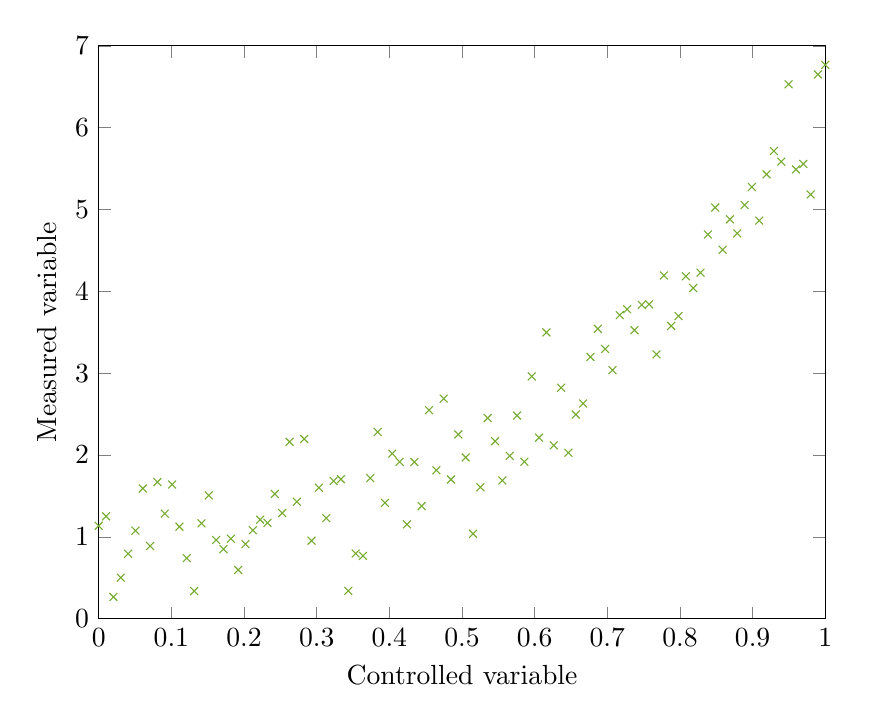
\begin{tikzpicture}

\begin{axis}[%
width=0.761\textwidth,
height=0.6\textwidth,
at={(0\textwidth,0\textwidth)},
scale only axis,
xmin=0,
xmax=1,
xlabel={Controlled variable},
ymin=0,
ymax=7,
ylabel={Measured variable},
axis background/.style={fill=white}
]
\addplot [color=mycolor1,mark size=2.0pt,only marks,mark=x,mark options={solid},forget plot]
  table[row sep=crcr]{%
0	1.1348243208583\\
0.0101010101010101	1.25066718379983\\
0.0202020202020202	0.265814534990681\\
0.0303030303030303	0.501443620387223\\
0.0404040404040404	0.792650094491283\\
0.0505050505050505	1.07594134463015\\
0.0606060606060606	1.59085902936445\\
0.0707070707070707	0.887323985428602\\
0.0808080808080808	1.66935315828504\\
0.0909090909090909	1.2830417321747\\
0.101010101010101	1.63964010570845\\
0.111111111111111	1.12383018697107\\
0.121212121212121	0.740267773623184\\
0.131313131313131	0.336861092429334\\
0.141414141414141	1.16477746407888\\
0.151515151515152	1.50639007889556\\
0.161616161616162	0.961532491139081\\
0.171717171717172	0.848797886459535\\
0.181818181818182	0.976908744250752\\
0.191919191919192	0.595667220167771\\
0.202020202020202	0.910910486977861\\
0.212121212121212	1.08123618761322\\
0.222222222222222	1.20947748015452\\
0.232323232323232	1.17039866186889\\
0.242424242424242	1.52449498941373\\
0.252525252525253	1.29084892850145\\
0.262626262626263	2.16140765753216\\
0.272727272727273	1.42949050169281\\
0.282828282828283	2.19569457569791\\
0.292929292929293	0.952768142342877\\
0.303030303030303	1.59941732609297\\
0.313131313131313	1.22878867706625\\
0.323232323232323	1.68273268144897\\
0.333333333333333	1.70437280523178\\
0.343434343434343	0.340162885446651\\
0.353535353535354	0.796460348337786\\
0.363636363636364	0.767346945232634\\
0.373737373737374	1.71773304601635\\
0.383838383838384	2.28197536666844\\
0.393939393939394	1.41466005871554\\
0.404040404040404	2.01657128322299\\
0.414141414141414	1.91669424420271\\
0.424242424242424	1.15281589577245\\
0.434343434343434	1.91328849589312\\
0.444444444444444	1.37576730829966\\
0.454545454545455	2.54826618060447\\
0.464646464646465	1.81354755013408\\
0.474747474747475	2.68883036644244\\
0.484848484848485	1.70062432900558\\
0.494949494949495	2.25153824042554\\
0.505050505050505	1.97046051602482\\
0.515151515151515	1.03729946755056\\
0.525252525252525	1.60504584806751\\
0.535353535353535	2.4516314559224\\
0.545454545454545	2.16865009804097\\
0.555555555555556	1.68891932113303\\
0.565656565656566	1.9887846581908\\
0.575757575757576	2.48193949192483\\
0.585858585858586	1.91741754395497\\
0.595959595959596	2.95970995960224\\
0.606060606060606	2.21177091099404\\
0.616161616161616	3.49805245178404\\
0.626262626262626	2.11680979614241\\
0.636363636363636	2.82110736917011\\
0.646464646464647	2.02743868031511\\
0.656565656565657	2.4942669438818\\
0.666666666666667	2.62930076842052\\
0.676767676767677	3.19817203212095\\
0.686868686868687	3.54190461781486\\
0.696969696969697	3.29619284049152\\
0.707070707070707	3.03632587120104\\
0.717171717171717	3.70933788652449\\
0.727272727272727	3.78161229147029\\
0.737373737373737	3.52471097304901\\
0.747474747474748	3.83455770018537\\
0.757575757575758	3.84156510313271\\
0.767676767676768	3.22984867115492\\
0.777777777777778	4.19322723565972\\
0.787878787878788	3.57692847085598\\
0.797979797979798	3.69765015806426\\
0.808080808080808	4.1841789617218\\
0.818181818181818	4.04008748370123\\
0.828282828282828	4.22812186933412\\
0.838383838383838	4.69398451179073\\
0.848484848484849	5.02409814076825\\
0.858585858585859	4.5082025936002\\
0.868686868686869	4.87966688348694\\
0.878787878787879	4.70749031401562\\
0.888888888888889	5.05444179366091\\
0.898989898989899	5.27485523897865\\
0.909090909090909	4.86386856322881\\
0.919191919191919	5.42941910663806\\
0.929292929292929	5.71452650214107\\
0.939393939393939	5.58440146428019\\
0.94949494949495	6.52975906004297\\
0.95959595959596	5.48949103313919\\
0.96969696969697	5.55653341937969\\
0.97979797979798	5.18380100303689\\
0.98989898989899	6.65006474115145\\
1	6.766874609807\\
};
\end{axis}
\end{tikzpicture}%
  \vfill
}

\frame{
  \frametitle{How to fit a model to the data?}
  We would like to fit the following model to the data:
  \[
    \hat{y} = a_1 + a_2x + a_3x^2 + a_4 x^3
  \]
  \vfill \pause
  First step: If we have $N$ data points, we could write the model as the product of a matrix and a vector:
  \begin{columns}\
    \column{0.6\textwidth}
      \[
      \begin{bmatrix}
      \hat{y}_1 \\
      \hat{y}_2 \\
      \hat{y}_3 \\
      \vdots \\
      \hat{y}_N
    \end{bmatrix}
    =
    \left. \begin{bmatrix}
      1 & x_1 & x_1^2 & x_1^3 \\
      1 & x_2 & x_2^2 & x_2^3 \\
      1 & x_3 & x_3^2 & x_3^3 \\
      \vdots  & \vdots  & \vdots  \\
      1 & x_N & x_N^2 & x_N^3
    \end{bmatrix}    
    \begin{bmatrix}
      a_1 \\
      a_2 \\
      a_3 \\
      a_4
    \end{bmatrix} \right.
      \]
    \column{0.4\textwidth}
    \tikz{\node[emphblock,text width=\columnwidth]{
    \begin{center}
    $
      \hat{y} = Xa
    $
    \end{center}
    $X$ is called the design matrix and $a$ are the fit parameters.
    }}
  \end{columns}
  \vfill
}

\frame{
  \frametitle{Residuals}
  Second step: work out the residuals for each data point:
  \[
    d_i = \left(y_i - \hat{y}_i\right)
  \]
  \pause
  Third step: work out the sum of squares of the residuals:
  \[
    \text{SSE} = \sum_i d_i^2 = \sum_i  \left(y_i - \hat{y}_i\right)^2
  \]
  This can be written using the dot-product operation:
    \[
    \text{SSE} = \sum_i d_i^2 = d \cdot d = d^T \cdot d = \left(y_i - \hat{y}_i\right)^T \cdot \left(y_i - \hat{y}_i\right)
  \]
}

\frame{
  \frametitle{Minimizing the sum of squares}
  Choose the parameter vector such that the sum of squares of the residuals is minimized; the partial derivative with respect to each parameter should be set to zero:
  \[
    \frac{\partial}{\partial a_i} \left[ \left(y - \left(Xa\right)^T\right)\left(y - Xa\right) \right]
  \]
  \pause
  In Matlab, we can solve our linear system $\hat{Y} = Xa$ simply by running \lstinline$a = np.linalg.solve(X,y)$.
  \pause
  \begin{itemize}
    \item If there are more data points ($N>4$), we can write an analogue, but maybe a consistent solution does not exist (the system is over specified).
    \item However, Python will find values for the vector a which minimize $\norm{y-aX}^2$ , so i.e. a least squares fit.
  \end{itemize}
}

% \frame{ 
%   \frametitle{Using Matlab's linear solver for fitting}
%   \begin{itemize}
%     \item If there are more data points ($N>4$), we can write an analogue, but maybe a consistent solution does not exist (the system is over specified).
%     \item However, matlab will find values for the vector a which minimize $\norm{y-aX}^2$ , so i.e. a least squares fit.
%   \end{itemize}
% }

\begin{frame}[fragile] 
  \frametitle{Fitting our problem: Least squares solver}
  As a follow-up of the script provided in slide~\ref{slidedatacreate}
  \begin{columns}[T]
    \column{0.5\textwidth}
    \begin{lstlisting}
import numpy as np

# Assuming x and y are defined previously
N = len(x)
X = np.zeros((N, 4))
X[:, 0] = 1
X[:, 1] = x
X[:, 2] = x**2
X[:, 3] = x**3
A = np.linalg.lstsq(X, y, rcond=None)[0]      

# y_fit = X@A 
    \end{lstlisting}
    \column{0.5\textwidth}
      % This file was created by matlab2tikz.
%
%The latest updates can be retrieved from
%  http://www.mathworks.com/matlabcentral/fileexchange/22022-matlab2tikz-matlab2tikz
%where you can also make suggestions and rate matlab2tikz.
%
\definecolor{mycolor1}{rgb}{0.00000,0.44700,0.74100}%
\definecolor{mycolor2}{rgb}{0.85000,0.32500,0.09800}%
%
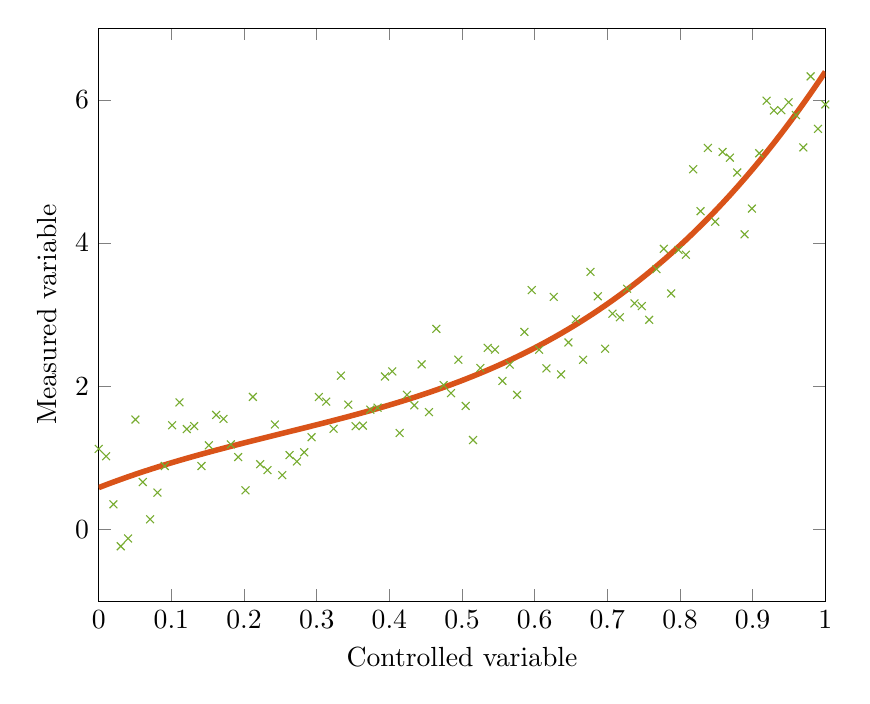
\begin{tikzpicture}

\begin{axis}[%
width=0.761\columnwidth,
height=0.6\columnwidth,
at={(0\columnwidth,0\columnwidth)},
scale only axis,
xmin=0,
xmax=1,
xlabel={Controlled variable},
ymin=-1,
ymax=7,
ylabel={Measured variable},
axis background/.style={fill=white}
]
\addplot [color=mycolor1,mark size=2.0pt,only marks,mark=x,mark options={solid},forget plot]
  table[row sep=crcr]{%
0	1.12469807930202\\
0.0101010101010101	1.02280166668951\\
0.0202020202020202	0.350939449073868\\
0.0303030303030303	-0.234638120472272\\
0.0404040404040404	-0.125824211743158\\
0.0505050505050505	1.53485805273449\\
0.0606060606060606	0.662228595963521\\
0.0707070707070707	0.142163381408442\\
0.0808080808080808	0.514325760703639\\
0.0909090909090909	0.886184325325323\\
0.101010101010101	1.45538141382297\\
0.111111111111111	1.77414284527193\\
0.121212121212121	1.40242389329148\\
0.131313131313131	1.44341498218508\\
0.141414141414141	0.885859449394921\\
0.151515151515152	1.17547542379997\\
0.161616161616162	1.5995984225065\\
0.171717171717172	1.54392845707063\\
0.181818181818182	1.18795915165698\\
0.191919191919192	1.01109225541317\\
0.202020202020202	0.546727611144681\\
0.212121212121212	1.85149900367413\\
0.222222222222222	0.911460427006403\\
0.232323232323232	0.828601284338836\\
0.242424242424242	1.46537439343075\\
0.252525252525253	0.758459251076779\\
0.262626262626263	1.03872005609328\\
0.272727272727273	0.950108795209328\\
0.282828282828283	1.0778761919738\\
0.292929292929293	1.28844117022709\\
0.303030303030303	1.84944852487809\\
0.313131313131313	1.78528145171749\\
0.323232323232323	1.4057875039612\\
0.333333333333333	2.1484354875216\\
0.343434343434343	1.74263282702635\\
0.353535353535354	1.4422817918771\\
0.363636363636364	1.44895581576432\\
0.373737373737374	1.67212006076371\\
0.383838383838384	1.70093662373074\\
0.393939393939394	2.1365873754442\\
0.404040404040404	2.20715336523681\\
0.414141414141414	1.34776471466763\\
0.424242424242424	1.88014589094255\\
0.434343434343434	1.73417289034226\\
0.444444444444444	2.30590903654202\\
0.454545454545455	1.63936303383897\\
0.464646464646465	2.80163458679989\\
0.474747474747475	2.01618432966198\\
0.484848484848485	1.90336004942572\\
0.494949494949495	2.3706671079675\\
0.505050505050505	1.72483930006325\\
0.515151515151515	1.24864161486139\\
0.525252525252525	2.25498057604476\\
0.535353535353535	2.536280883908\\
0.545454545454545	2.51195794239466\\
0.555555555555556	2.07456349976771\\
0.565656565656566	2.30181769243691\\
0.575757575757576	1.88037722329776\\
0.585858585858586	2.75883560272925\\
0.595959595959596	3.34336135129164\\
0.606060606060606	2.51031326006862\\
0.616161616161616	2.24954462659987\\
0.626262626262626	3.24794169386657\\
0.636363636363636	2.16523110579606\\
0.646464646464647	2.61168297908951\\
0.656565656565657	2.93473299609728\\
0.666666666666667	2.36927374312803\\
0.676767676767677	3.59731207093502\\
0.686868686868687	3.25664421173762\\
0.696969696969697	2.52352672096175\\
0.707070707070707	3.01365675628849\\
0.717171717171717	2.96384122265525\\
0.727272727272727	3.36214903103335\\
0.737373737373737	3.15644471241314\\
0.747474747474748	3.11901092988185\\
0.757575757575758	2.92755684095319\\
0.767676767676768	3.63537445215587\\
0.777777777777778	3.91853689313825\\
0.787878787878788	3.29583824281356\\
0.797979797979798	3.90512820774034\\
0.808080808080808	3.83687384026147\\
0.818181818181818	5.03022334538949\\
0.828282828282828	4.44448985140307\\
0.838383838383838	5.32825444340593\\
0.848484848484849	4.29736936458515\\
0.858585858585859	5.27209415952454\\
0.868686868686869	5.19206091917515\\
0.878787878787879	4.98454589099849\\
0.888888888888889	4.1214094788034\\
0.898989898989899	4.48120393467531\\
0.909090909090909	5.25372695563257\\
0.919191919191919	5.98740371535861\\
0.929292929292929	5.85044844176157\\
0.939393939393939	5.85533130947701\\
0.94949494949495	5.96662989986236\\
0.95959595959596	5.78809692669365\\
0.96969696969697	5.33518109654205\\
0.97979797979798	6.32739472598414\\
0.98989898989899	5.59498111585168\\
1	5.9352339503879\\
};
\addplot [color=mycolor2,solid,line width=2.0pt,forget plot]
  table[row sep=crcr]{%
0	0.584384979074576\\
0.0101010101010101	0.62382829973825\\
0.0202020202020202	0.662149819770938\\
0.0303030303030303	0.699396363234128\\
0.0404040404040404	0.73561475418931\\
0.0505050505050505	0.770851816697972\\
0.0606060606060606	0.805154374821606\\
0.0707070707070707	0.838569252621699\\
0.0808080808080808	0.871143274159741\\
0.0909090909090909	0.902923263497222\\
0.101010101010101	0.93395604469563\\
0.111111111111111	0.964288441816455\\
0.121212121212121	0.993967278921188\\
0.131313131313131	1.02303938007132\\
0.141414141414141	1.05155156932833\\
0.151515151515152	1.07955067075372\\
0.161616161616162	1.10708350840897\\
0.171717171717172	1.13419690635557\\
0.181818181818182	1.16093768865502\\
0.191919191919192	1.1873526793688\\
0.202020202020202	1.2134887025584\\
0.212121212121212	1.23939258228531\\
0.222222222222222	1.26511114261102\\
0.232323232323232	1.29069120759702\\
0.242424242424242	1.3161796013048\\
0.252525252525253	1.34162314779585\\
0.262626262626263	1.36706867113165\\
0.272727272727273	1.3925629953737\\
0.282828282828283	1.41815294458349\\
0.292929292929293	1.4438853428225\\
0.303030303030303	1.46980701415223\\
0.313131313131313	1.49596478263416\\
0.323232323232323	1.52240547232978\\
0.333333333333333	1.54917590730059\\
0.343434343434343	1.57632291160806\\
0.353535353535354	1.6038933093137\\
0.363636363636364	1.631933924479\\
0.373737373737374	1.66049158116543\\
0.383838383838384	1.68961310343449\\
0.393939393939394	1.71934531534766\\
0.404040404040404	1.74973504096645\\
0.414141414141414	1.78082910435234\\
0.424242424242424	1.81267432956681\\
0.434343434343434	1.84531754067135\\
0.444444444444444	1.87880556172747\\
0.454545454545455	1.91318521679664\\
0.464646464646465	1.94850332994035\\
0.474747474747475	1.98480672522009\\
0.484848484848485	2.02214222669736\\
0.494949494949495	2.06055665843364\\
0.505050505050505	2.10009684449042\\
0.515151515151515	2.14080960892919\\
0.525252525252525	2.18274177581145\\
0.535353535353535	2.22594016919867\\
0.545454545454545	2.27045161315235\\
0.555555555555556	2.31632293173398\\
0.565656565656566	2.36360094900505\\
0.575757575757576	2.41233248902704\\
0.585858585858586	2.46256437586145\\
0.595959595959596	2.51434343356977\\
0.606060606060606	2.56771648621348\\
0.616161616161616	2.62273035785407\\
0.626262626262626	2.67943187255304\\
0.636363636363636	2.73786785437187\\
0.646464646464647	2.79808512737206\\
0.656565656565657	2.86013051561508\\
0.666666666666667	2.92405084316244\\
0.676767676767677	2.98989293407562\\
0.686868686868687	3.0577036124161\\
0.696969696969697	3.12752970224539\\
0.707070707070707	3.19941802762496\\
0.717171717171717	3.27341541261631\\
0.727272727272727	3.34956868128093\\
0.737373737373737	3.42792465768031\\
0.747474747474748	3.50853016587593\\
0.757575757575758	3.59143202992928\\
0.767676767676768	3.67667707390186\\
0.777777777777778	3.76431212185516\\
0.787878787878788	3.85438399785065\\
0.797979797979798	3.94693952594985\\
0.808080808080808	4.04202553021422\\
0.818181818181818	4.13968883470526\\
0.828282828282828	4.23997626348446\\
0.838383838383838	4.34293464061332\\
0.848484848484849	4.44861079015331\\
0.858585858585859	4.55705153616593\\
0.868686868686869	4.66830370271267\\
0.878787878787879	4.78241411385501\\
0.888888888888889	4.89942959365445\\
0.898989898989899	5.01939696617248\\
0.909090909090909	5.14236305547059\\
0.919191919191919	5.26837468561025\\
0.929292929292929	5.39747868065298\\
0.939393939393939	5.52972186466024\\
0.94949494949495	5.66515106169354\\
0.95959595959596	5.80381309581436\\
0.96969696969697	5.94575479108419\\
0.97979797979798	6.09102297156452\\
0.98989898989899	6.23966446131684\\
1	6.39172608440264\\
};
\end{axis}
\end{tikzpicture}%
  \end{columns}
\end{frame}


\begin{frame}[fragile] 
  \frametitle{Fitting our problem: Excel}
    \begin{itemize}
      \item Create a column with the independent and dependent data series ($x$ and $y$)
      \item Create a column that computes $\hat{y}$, keeping the coefficients as separate cells
      \item Compute the sum of squares of the residuals (another column, sum the results)
      \item Use the solver to minimize this sum, modifying the coefficient cells
      \item Note: regression in Excel + display equation is dangerous if you choose the 'line' plot (use scatter if you can)
    \end{itemize}
\end{frame}

\begin{frame}[fragile] 
  \frametitle{How good is the model?}
  % This file was created by matlab2tikz.
%
%The latest updates can be retrieved from
%  http://www.mathworks.com/matlabcentral/fileexchange/22022-matlab2tikz-matlab2tikz
%where you can also make suggestions and rate matlab2tikz.
%
\definecolor{mycolor1}{rgb}{0.00000,0.44700,0.74100}%
%
\begin{tikzpicture}

\begin{axis}[%
width=0.856\textwidth,
height=0.3\textheight,
at={(0\textwidth,0\textheight)},
scale only axis,
xmin=0,
xmax=1,
xlabel={Controlled variable},
ymin=-2,
ymax=2,
ylabel={Absolute deviation},
axis background/.style={fill=white},
title style={font=\bfseries},
title={Mean residual: -7.1276e-16},
legend style={legend cell align=left,align=left,draw=white!15!black}
]
\addplot[ycomb,color=mycolor1,solid,mark size=2.0pt,mark=o,mark options={solid},forget plot] plot table[row sep=crcr] {%
0	-0.163601677546173\\
0.0101010101010101	0.507255617941878\\
0.0202020202020202	-1.517204055749\\
0.0303030303030303	0.0643856726685146\\
0.0404040404040404	-0.187049888753044\\
0.0505050505050505	-0.980803869422559\\
0.0606060606060606	-0.525063168952326\\
0.0707070707070707	-0.119027117523669\\
0.0808080808080808	1.51603763709065\\
0.0909090909090909	1.12800237868348\\
0.101010101010101	-0.91593326385323\\
0.111111111111111	1.2914953953239\\
0.121212121212121	0.151071811491146\\
0.131313131313131	-0.229493652311215\\
0.141414141414141	0.172412837345806\\
0.151515151515152	-0.275075059206132\\
0.161616161616162	-0.222923168813328\\
0.171717171717172	0.595128762856934\\
0.181818181818182	0.565333543330339\\
0.191919191919192	0.579369697885556\\
0.202020202020202	0.215915571468414\\
0.212121212121212	-0.71473115495332\\
0.222222222222222	0.25594418948787\\
0.232323232323232	0.720237789027717\\
0.242424242424242	0.156860500889024\\
0.252525252525253	0.436567250123936\\
0.262626262626263	0.288999566910829\\
0.272727272727273	-0.220282614019045\\
0.282828282828283	0.08381449065582\\
0.292929292929293	-0.451746207981299\\
0.303030303030303	0.390700442102595\\
0.313131313131313	-0.622818531921597\\
0.323232323232323	-0.579882881690158\\
0.333333333333333	-0.4467237760178\\
0.343434343434343	-1.51099042055391\\
0.353535353535354	0.683136229026347\\
0.363636363636364	0.129019574926726\\
0.373737373737374	-0.408862363923595\\
0.383838383838384	0.655643291532526\\
0.393939393939394	-0.883641759279032\\
0.404040404040404	-0.0776366739145484\\
0.414141414141414	-0.146109734899402\\
0.424242424242424	0.135122997537032\\
0.434343434343434	0.13264684107515\\
0.444444444444444	-0.455716960873263\\
0.454545454545455	-0.0379741875680402\\
0.464646464646465	-0.105221111146472\\
0.474747474747475	0.291092922815414\\
0.484848484848485	0.523762404307071\\
0.494949494949495	0.531541386952305\\
0.505050505050505	-0.455246159391748\\
0.515151515151515	0.0148511232032731\\
0.525252525252525	-0.631364338078018\\
0.535353535353535	-0.58158683338767\\
0.545454545454545	-0.0288295580573106\\
0.555555555555556	0.740319511266238\\
0.565656565656566	-0.411426198654404\\
0.575757575757576	0.158507183148339\\
0.585858585858586	-0.140539320895918\\
0.595959595959596	0.530405605522088\\
0.606060606060606	-0.573274935654142\\
0.616161616161616	-0.0128638929282161\\
0.626262626262626	0.246807003501153\\
0.636363636363636	0.520636142157868\\
0.646464646464647	0.742341411036678\\
0.656565656565657	0.0132378172127825\\
0.666666666666667	-0.775338292602044\\
0.676767676767677	-0.400346151591929\\
0.686868686868687	-0.559459435592979\\
0.696969696969697	1.14728093428305\\
0.707070707070707	-0.334818032572183\\
0.717171717171717	0.348177048034943\\
0.727272727272727	-0.120674221468823\\
0.737373737373737	0.421492721276928\\
0.747474747474748	-0.403313070398987\\
0.757575757575758	-0.719811865410699\\
0.767676767676768	-0.727351772379763\\
0.777777777777778	0.230764683015058\\
0.787878787878788	-0.0988548778151972\\
0.797979797979798	-0.104680169032075\\
0.808080808080808	0.706879894016713\\
0.818181818181818	0.147275086436078\\
0.828282828282828	0.105041811327639\\
0.838383838383838	0.805049986615106\\
0.848484848484849	-0.385542140154703\\
0.858585858585859	0.370935149174467\\
0.868686868686869	0.446556301331418\\
0.878787878787879	-0.0859834320544364\\
0.888888888888889	0.151059209948147\\
0.898989898989899	-0.531844193632515\\
0.909090909090909	-0.514525967749829\\
0.919191919191919	0.120794941005622\\
0.929292929292929	0.438941739592955\\
0.939393939393939	1.38058293693505\\
0.94949494949495	-0.235004523435661\\
0.95959595959596	0.20330620711245\\
0.96969696969697	0.0802052141435237\\
0.97979797979798	-0.832619983514173\\
0.98989898989899	-0.0725097689192244\\
1	-0.736626028509808\\
};
\addplot [color=black,solid,forget plot]
  table[row sep=crcr]{%
0	0\\
1	0\\
};
\end{axis}
\end{tikzpicture}%

  \begin{itemize}
    \item For a model to make sense the data points should be scattered randomly around the model predictions, the mean of the residuals $d$ should be zero: $d_i = \left( y_i - \hat{y}_i\right)$
    \item It’s always good to check if the residuals are not correlated with the measured values, if that is the case, it can indicate that your model is wrong.
  \end{itemize}
\end{frame}

\section{Regression}
\subsection*{}
\againframe<2>{contents_opt}
\begin{frame}[fragile] 
  \frametitle{Regression coefficients}
    \begin{itemize}
    \item Variance measured in the data (y) is:
    \[
      \sigma^2_y = \frac{1}{N} \sum_i \left (y_i - \overline{y}\right)^2
    \]
    \item Variance of the residuals is:
    \[
      \sigma^2_\text{error} = \frac{1}{N} \sum_i \left (d_i\right)^2
    \]
        \item Variance in the model is:
    \[
      \sigma^2_\text{model} = \frac{1}{N} \sum_i \left (\hat{y}_i - \overline{\hat{y}}\right)^2
    \]
  \end{itemize}
\end{frame}

\begin{frame}[fragile] 
  \frametitle{Regression coefficients}
  Given that the error is uncorrelated we can state that:
    \[
      \sigma^2_y = \sigma^2_\text{error}+\sigma^2_\text{model}
    \]
    \[
      R^2 = \frac{\sigma^2_\text{model}}{\sigma^2_y} = 1 - \frac{\sigma^2_\text{error}}{\sigma^2_y}
    \]
    \[
      R^2 = 1 - \frac{\text{SSE}}{\text{SST}}
    \]
    \begin{itemize}
      \item SSE: Sum of errors (residuals) squared (difference between data and model)
      \item SST: Total sum of squares (variance of the data)
      \item SSR: Sum of squares (model)
   \end{itemize}
\end{frame}

% \begin{frame}[fragile] 
%   \frametitle{Regression coefficients}
%     \begin{itemize}
%       \item An uncorrellated error ($\overline{d} \rightarrow 0$) means that SSE, SST and SSR will have $\chi^2$ -distributions and the ratios will have an F-distribution. If SSR/SSE is large, the model is good!
%       \item There is a chance that the model is rubbish, but that SSR/SSE will yield a good value, Analysis of Variance (ANOVA) will be a good tool to calculate the probability of such a thing happening!
%    \end{itemize}
% \end{frame}

\begin{frame}[fragile] 
  \frametitle{Back to the example}
  \begin{columns}
    \column{0.4\textwidth}
      \begin{center}
        The statistics: \\ \vskip1em
        % \begin{tabular}{lc}
 & Value \\ 
\hline$N$   & 100 \\ 
SSE   & 20.310 \\ 
SST   & 894.115 \\ 
SSR   & 914.425 \\ 
$R^2$ & 0.977 \\ 
\hline\end{tabular}

        \begin{tabular}{lc}
          & Value \\ 
         \hline$N$   & 100 \\ 
         SSE   & 32.042 \\ 
         SST   & 896.907 \\ 
         SSR   & 928.950 \\ 
         $R^2$ & 0.964 \\ 
         \hline\end{tabular}
      \end{center}
    \column{0.6\textwidth}
      % This file was created by matlab2tikz.
%
%The latest updates can be retrieved from
%  http://www.mathworks.com/matlabcentral/fileexchange/22022-matlab2tikz-matlab2tikz
%where you can also make suggestions and rate matlab2tikz.
%
\definecolor{mycolor1}{rgb}{0.00000,0.44700,0.74100}%
\definecolor{mycolor2}{rgb}{0.85000,0.32500,0.09800}%
%
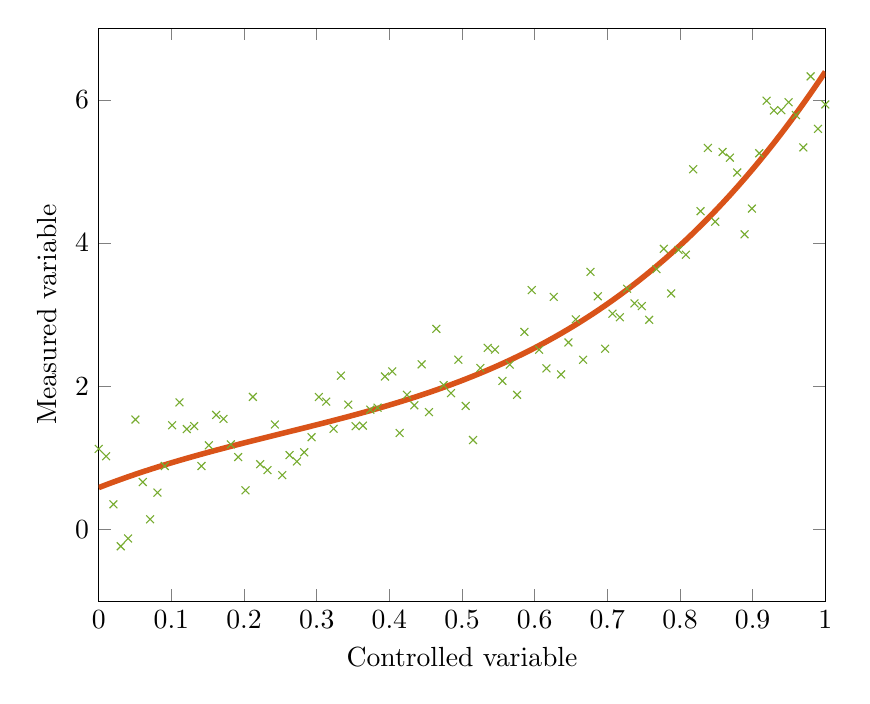
\begin{tikzpicture}

\begin{axis}[%
width=0.761\columnwidth,
height=0.6\columnwidth,
at={(0\columnwidth,0\columnwidth)},
scale only axis,
xmin=0,
xmax=1,
xlabel={Controlled variable},
ymin=-1,
ymax=7,
ylabel={Measured variable},
axis background/.style={fill=white}
]
\addplot [color=mycolor1,mark size=2.0pt,only marks,mark=x,mark options={solid},forget plot]
  table[row sep=crcr]{%
0	1.12469807930202\\
0.0101010101010101	1.02280166668951\\
0.0202020202020202	0.350939449073868\\
0.0303030303030303	-0.234638120472272\\
0.0404040404040404	-0.125824211743158\\
0.0505050505050505	1.53485805273449\\
0.0606060606060606	0.662228595963521\\
0.0707070707070707	0.142163381408442\\
0.0808080808080808	0.514325760703639\\
0.0909090909090909	0.886184325325323\\
0.101010101010101	1.45538141382297\\
0.111111111111111	1.77414284527193\\
0.121212121212121	1.40242389329148\\
0.131313131313131	1.44341498218508\\
0.141414141414141	0.885859449394921\\
0.151515151515152	1.17547542379997\\
0.161616161616162	1.5995984225065\\
0.171717171717172	1.54392845707063\\
0.181818181818182	1.18795915165698\\
0.191919191919192	1.01109225541317\\
0.202020202020202	0.546727611144681\\
0.212121212121212	1.85149900367413\\
0.222222222222222	0.911460427006403\\
0.232323232323232	0.828601284338836\\
0.242424242424242	1.46537439343075\\
0.252525252525253	0.758459251076779\\
0.262626262626263	1.03872005609328\\
0.272727272727273	0.950108795209328\\
0.282828282828283	1.0778761919738\\
0.292929292929293	1.28844117022709\\
0.303030303030303	1.84944852487809\\
0.313131313131313	1.78528145171749\\
0.323232323232323	1.4057875039612\\
0.333333333333333	2.1484354875216\\
0.343434343434343	1.74263282702635\\
0.353535353535354	1.4422817918771\\
0.363636363636364	1.44895581576432\\
0.373737373737374	1.67212006076371\\
0.383838383838384	1.70093662373074\\
0.393939393939394	2.1365873754442\\
0.404040404040404	2.20715336523681\\
0.414141414141414	1.34776471466763\\
0.424242424242424	1.88014589094255\\
0.434343434343434	1.73417289034226\\
0.444444444444444	2.30590903654202\\
0.454545454545455	1.63936303383897\\
0.464646464646465	2.80163458679989\\
0.474747474747475	2.01618432966198\\
0.484848484848485	1.90336004942572\\
0.494949494949495	2.3706671079675\\
0.505050505050505	1.72483930006325\\
0.515151515151515	1.24864161486139\\
0.525252525252525	2.25498057604476\\
0.535353535353535	2.536280883908\\
0.545454545454545	2.51195794239466\\
0.555555555555556	2.07456349976771\\
0.565656565656566	2.30181769243691\\
0.575757575757576	1.88037722329776\\
0.585858585858586	2.75883560272925\\
0.595959595959596	3.34336135129164\\
0.606060606060606	2.51031326006862\\
0.616161616161616	2.24954462659987\\
0.626262626262626	3.24794169386657\\
0.636363636363636	2.16523110579606\\
0.646464646464647	2.61168297908951\\
0.656565656565657	2.93473299609728\\
0.666666666666667	2.36927374312803\\
0.676767676767677	3.59731207093502\\
0.686868686868687	3.25664421173762\\
0.696969696969697	2.52352672096175\\
0.707070707070707	3.01365675628849\\
0.717171717171717	2.96384122265525\\
0.727272727272727	3.36214903103335\\
0.737373737373737	3.15644471241314\\
0.747474747474748	3.11901092988185\\
0.757575757575758	2.92755684095319\\
0.767676767676768	3.63537445215587\\
0.777777777777778	3.91853689313825\\
0.787878787878788	3.29583824281356\\
0.797979797979798	3.90512820774034\\
0.808080808080808	3.83687384026147\\
0.818181818181818	5.03022334538949\\
0.828282828282828	4.44448985140307\\
0.838383838383838	5.32825444340593\\
0.848484848484849	4.29736936458515\\
0.858585858585859	5.27209415952454\\
0.868686868686869	5.19206091917515\\
0.878787878787879	4.98454589099849\\
0.888888888888889	4.1214094788034\\
0.898989898989899	4.48120393467531\\
0.909090909090909	5.25372695563257\\
0.919191919191919	5.98740371535861\\
0.929292929292929	5.85044844176157\\
0.939393939393939	5.85533130947701\\
0.94949494949495	5.96662989986236\\
0.95959595959596	5.78809692669365\\
0.96969696969697	5.33518109654205\\
0.97979797979798	6.32739472598414\\
0.98989898989899	5.59498111585168\\
1	5.9352339503879\\
};
\addplot [color=mycolor2,solid,line width=2.0pt,forget plot]
  table[row sep=crcr]{%
0	0.584384979074576\\
0.0101010101010101	0.62382829973825\\
0.0202020202020202	0.662149819770938\\
0.0303030303030303	0.699396363234128\\
0.0404040404040404	0.73561475418931\\
0.0505050505050505	0.770851816697972\\
0.0606060606060606	0.805154374821606\\
0.0707070707070707	0.838569252621699\\
0.0808080808080808	0.871143274159741\\
0.0909090909090909	0.902923263497222\\
0.101010101010101	0.93395604469563\\
0.111111111111111	0.964288441816455\\
0.121212121212121	0.993967278921188\\
0.131313131313131	1.02303938007132\\
0.141414141414141	1.05155156932833\\
0.151515151515152	1.07955067075372\\
0.161616161616162	1.10708350840897\\
0.171717171717172	1.13419690635557\\
0.181818181818182	1.16093768865502\\
0.191919191919192	1.1873526793688\\
0.202020202020202	1.2134887025584\\
0.212121212121212	1.23939258228531\\
0.222222222222222	1.26511114261102\\
0.232323232323232	1.29069120759702\\
0.242424242424242	1.3161796013048\\
0.252525252525253	1.34162314779585\\
0.262626262626263	1.36706867113165\\
0.272727272727273	1.3925629953737\\
0.282828282828283	1.41815294458349\\
0.292929292929293	1.4438853428225\\
0.303030303030303	1.46980701415223\\
0.313131313131313	1.49596478263416\\
0.323232323232323	1.52240547232978\\
0.333333333333333	1.54917590730059\\
0.343434343434343	1.57632291160806\\
0.353535353535354	1.6038933093137\\
0.363636363636364	1.631933924479\\
0.373737373737374	1.66049158116543\\
0.383838383838384	1.68961310343449\\
0.393939393939394	1.71934531534766\\
0.404040404040404	1.74973504096645\\
0.414141414141414	1.78082910435234\\
0.424242424242424	1.81267432956681\\
0.434343434343434	1.84531754067135\\
0.444444444444444	1.87880556172747\\
0.454545454545455	1.91318521679664\\
0.464646464646465	1.94850332994035\\
0.474747474747475	1.98480672522009\\
0.484848484848485	2.02214222669736\\
0.494949494949495	2.06055665843364\\
0.505050505050505	2.10009684449042\\
0.515151515151515	2.14080960892919\\
0.525252525252525	2.18274177581145\\
0.535353535353535	2.22594016919867\\
0.545454545454545	2.27045161315235\\
0.555555555555556	2.31632293173398\\
0.565656565656566	2.36360094900505\\
0.575757575757576	2.41233248902704\\
0.585858585858586	2.46256437586145\\
0.595959595959596	2.51434343356977\\
0.606060606060606	2.56771648621348\\
0.616161616161616	2.62273035785407\\
0.626262626262626	2.67943187255304\\
0.636363636363636	2.73786785437187\\
0.646464646464647	2.79808512737206\\
0.656565656565657	2.86013051561508\\
0.666666666666667	2.92405084316244\\
0.676767676767677	2.98989293407562\\
0.686868686868687	3.0577036124161\\
0.696969696969697	3.12752970224539\\
0.707070707070707	3.19941802762496\\
0.717171717171717	3.27341541261631\\
0.727272727272727	3.34956868128093\\
0.737373737373737	3.42792465768031\\
0.747474747474748	3.50853016587593\\
0.757575757575758	3.59143202992928\\
0.767676767676768	3.67667707390186\\
0.777777777777778	3.76431212185516\\
0.787878787878788	3.85438399785065\\
0.797979797979798	3.94693952594985\\
0.808080808080808	4.04202553021422\\
0.818181818181818	4.13968883470526\\
0.828282828282828	4.23997626348446\\
0.838383838383838	4.34293464061332\\
0.848484848484849	4.44861079015331\\
0.858585858585859	4.55705153616593\\
0.868686868686869	4.66830370271267\\
0.878787878787879	4.78241411385501\\
0.888888888888889	4.89942959365445\\
0.898989898989899	5.01939696617248\\
0.909090909090909	5.14236305547059\\
0.919191919191919	5.26837468561025\\
0.929292929292929	5.39747868065298\\
0.939393939393939	5.52972186466024\\
0.94949494949495	5.66515106169354\\
0.95959595959596	5.80381309581436\\
0.96969696969697	5.94575479108419\\
0.97979797979798	6.09102297156452\\
0.98989898989899	6.23966446131684\\
1	6.39172608440264\\
};
\end{axis}
\end{tikzpicture}%
  \end{columns}
\end{frame}

\section{Fitting numerical models}
\subsection*{}
\againframe<2>{contents_opt}
\begin{frame}[fragile]
  \frametitle{Curve fitting from command line: scipy.optimize.curve\_fit}
  Python offers various non-linear parameter and curve fitting tools that can be run from the command line. The function \lstinline$curve_fit$ from the \lstinline$scipy.optimize$ module allows to fit a model to a given dataset. Again, based on the data generated in slide~\ref{slidedatacreate}:
    \begin{lstlisting}[language=Python,basicstyle=\tiny]
from scipy.optimize import curve_fit

# Initial guess of coefficients
a0 = [1, 2, 1, 3]

# Define the model function
def curve_fit_model(xdata, a1, a2, a3, a4):
    return a1*xdata**3 + a2*xdata**2 + a3*xdata + a4

# Perform fitting, store resulting coeffs in a_fit
a_fit, _ = curve_fit(curve_fit_model, x, y, p0=a0)

# Run the model once more, with fitted coefficients
y_model = curve_fit_model(x, *a_fit)

plt.plot(x, y_model, '-r')
plt.show()
    \end{lstlisting}
    In the Python translation, the model function takes individual parameters separately rather than as an array, and we use the unpacking syntax (\lstinline$*$) to pass the fitted parameters when generating the \lstinline$y_model$ data.
  \end{frame}
  

  \begin{frame}[fragile] 
    \frametitle{Dynamic fitting of non-linear equations}
    You may encounter situations where the model data is slightly more complicated to obtain (e.g., a numerical model based on ODEs where coefficients are unknown), or you want to perform fitting of multiple functions/coefficients, or just want to automate things via scripts. Python's Scipy library gives access to powerful functions such as \lstinline$least_squares$ and \lstinline$curve_fit$.
  \end{frame}
    
  \begin{frame}[fragile] 
    \frametitle{General use of scipy.optimize.least\_squares}
    \begin{lstlisting}[language=Python]
from scipy.optimize import least_squares

result = least_squares(fun, k0, bounds=(lb, ub), xtol=1.0E-6, max_nfev=1000)
    \end{lstlisting}
    \begin{itemize}
      \item \lstinline$fun$ is a function handle to the fit criterion (e.g., \lstinline$myFitCrit$). The fit criterion function \lstinline$myFitCrit$ should return the residuals vector, e.g., $d_i = \left(y_i - \hat{y}_i\right)$. Here, $y_i$ would again be the measurement data and $\hat{y}$ the solution computed by a model.
      \item \lstinline$k0$ is the initial guess for the fitting coefficient (or: array of initial guesses when fitting multiple coefficients).
      \item \lstinline$lb$ and \lstinline$ub$ are the lower and upper boundaries for \lstinline$k0$. These should both be the size of the \lstinline$k0$-array.
      \item Use arguments such as \lstinline$xtol$ and \lstinline$max_nfev$ for more fine-grained control on the fit procedure. 
    \end{itemize}  
  \end{frame}
  
  
  \begin{frame}[fragile] 
  \frametitle{General use of scipy.optimize.curve\_fit}
  \begin{lstlisting}[language=Python]
from scipy.optimize import curve_fit

popt, pcov = curve_fit(fun, xdata, ydata, p0=k0, bounds=(lb, ub))
  \end{lstlisting}
  \begin{itemize}
    \item \lstinline$fun$ is the model function that you want to fit to your data. It takes the independent variable as the first argument and the parameters to fit as separate remaining arguments.
    \item \lstinline$xdata$ and \lstinline$ydata$ are the data points that you are fitting the model function to.
    \item \lstinline$k0$ is the initial guess for the parameters to be fitted.
    \item \lstinline$lb$ and \lstinline$ub$ are the lower and upper bounds for the parameters, respectively.
    \item \lstinline$popt$ will contain the optimized parameters, and \lstinline$pcov$ will contain the covariance matrix, which can give you an idea of the uncertainties of the estimates.
  \end{itemize}  
  \end{frame}
    

  \begin{frame}[fragile] 
    \frametitle{Example use of scipy.optimize.curve\_fit}
    We have experimental data stored in a file, possibly in a .csv or .txt format, containing $T$ and $U$ data. We want to fit a model with coefficients $k_1$ and $k_2$ with the following structure:
    \[
      \frac{du}{dt} = -k_1 u + k_2
    \]
    \pause
    \begin{itemize}
      \item First, we define a function that describes our model:
      \begin{lstlisting}[language=Python,basicstyle=\scriptsize]
from scipy.integrate import odeint

def simpleode(u, t, k1, k2):
    dudt = -k1*u + k2
    return dudt
      \end{lstlisting}
      Note that we supply the coefficients \(k_1\) and \(k_2\) as arguments to the function.
      \pause
      \item We create a fit criterion function:
      \begin{lstlisting}[language=Python,basicstyle=\scriptsize]
def fitcrit(t, k1, k2):
    u0 = 1.0
    u = odeint(simpleode, u0, t, args=(k1, k2))
    return u.ravel()
      \end{lstlisting}
    \end{itemize}
    \end{frame}
    
    \begin{frame}[fragile] 
    \frametitle{Example use of scipy.optimize.curve\_fit}
    Now let's make a script that uses \lstinline$curve_fit$ to yield k-values fitted to our dataset:
    \pause
    \begin{lstlisting}[language=Python,basicstyle=\scriptsize]
from scipy.optimize import curve_fit
import numpy as np

# Load your data here (adjust as necessary)
T, U = np.loadtxt('./scripts/used_by_students/lecture_archive_regression_optim/tudataset1.txt', unpack=True, skiprows=1)

# Initial guesses for model parameters
k0 = [1.0, 1.0]

# Perform the curve fitting
params, params_covariance = curve_fit(fitcrit, T, U, p0=k0)

print('Fitted coefficients:', params)
    \end{lstlisting}
    Our fitted coefficients are stored in \lstinline|params|. The \lstinline|params_covariance| gives an estimate of the covariance of the estimated parameters, offering an insight into the uncertainty of the fit.
    \end{frame}      

\begin{frame}[fragile] 
  \frametitle{Example use of lsqnonlin}
  \centering% This file was created by matlab2tikz.
%
%The latest updates can be retrieved from
%  http://www.mathworks.com/matlabcentral/fileexchange/22022-matlab2tikz-matlab2tikz
%where you can also make suggestions and rate matlab2tikz.
%
\definecolor{mycolor1}{rgb}{0.00000,0.44700,0.74100}%
\definecolor{mycolor2}{rgb}{0.85000,0.32500,0.09800}%
%
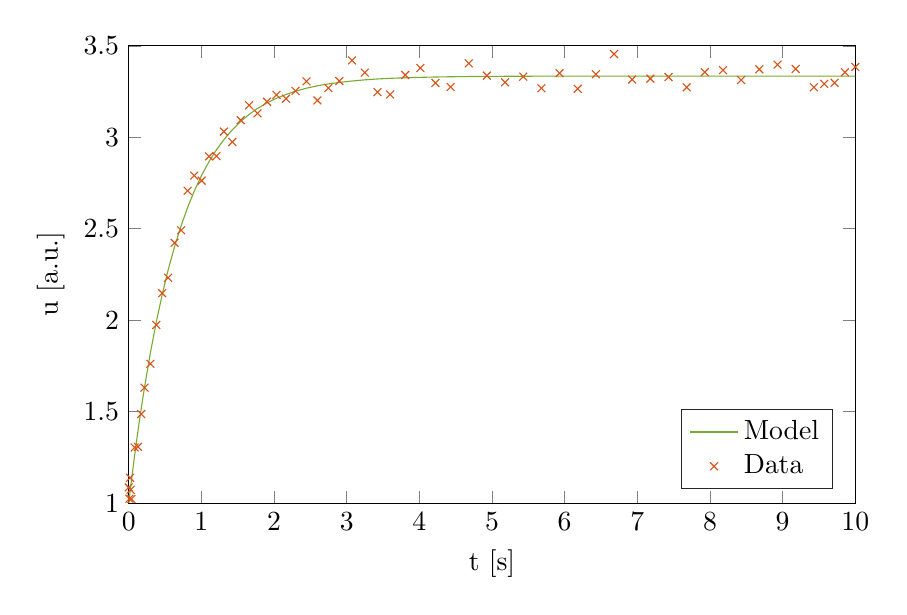
\begin{tikzpicture}

\begin{axis}[%
width=0.761\textwidth,
height=0.479\textwidth,
at={(0\textwidth,0\textwidth)},
scale only axis,
xmin=0,
xmax=10,
xlabel={t [s]},
ymin=1,
ymax=3.5,
ylabel={u [a.u.]},
axis background/.style={fill=white},
legend style={at={(0.97,0.03)},anchor=south east,legend cell align=left,align=left,draw=white!15!black}
]
\addplot [color=mycolor1,solid]
  table[row sep=crcr]{%
0	1\\
0.00905653252834922	1.03054168302136\\
0.0181130650566984	1.06068382326816\\
0.0271695975850477	1.09043164664039\\
0.0362261301133969	1.11979031057633\\
0.081508792755143	1.26092345274857\\
0.126791455396889	1.39306594927116\\
0.172074118038635	1.51678546295645\\
0.217356780680381	1.63261805453274\\
0.298396196924869	1.82181187581453\\
0.379435613169357	1.99015039516732\\
0.460475029413845	2.13981339624173\\
0.541514445658334	2.27271706424037\\
0.631466584260591	2.40281030512571\\
0.721418722862849	2.51681966031717\\
0.811370861465107	2.61692196689085\\
0.901323000067364	2.70501251052284\\
1.00352869986689	2.7921726339636\\
1.10573439966641	2.86719163742732\\
1.20794009946594	2.931668523432\\
1.31014579926546	2.98711739415208\\
1.42559217441384	3.04068110770477\\
1.54103854956222	3.0862630279324\\
1.65648492471059	3.12487214459275\\
1.77193129985897	3.15739226598622\\
1.90306590920505	3.18805211229742\\
2.03420051855113	3.2132454513137\\
2.1653351278972	3.23421332725045\\
2.29646973724328	3.25181115881682\\
2.44689896166169	3.26831178623415\\
2.5973281860801	3.2814117262679\\
2.74775741049851	3.29172422399088\\
2.89818663491692	3.29991499200663\\
3.07327320345979	3.30767939369721\\
3.24835977200267	3.31390119562681\\
3.42344634054554	3.3186959043631\\
3.59853290908841	3.32227204253787\\
3.80632677403043	3.32532068973421\\
4.01412063897244	3.32763104247754\\
4.22191450391446	3.32949871940074\\
4.42970836885647	3.33087906360708\\
4.67970836885647	3.33201168193161\\
4.92970836885647	3.33276268010813\\
5.17970836885647	3.33334038810328\\
5.42970836885647	3.33375027545222\\
5.67970836885647	3.33402047069873\\
5.92970836885647	3.33419962737759\\
6.17970836885647	3.33433744428447\\
6.42970836885647	3.33443522622115\\
6.67970836885647	3.33449968347887\\
6.92970836885647	3.33454242275119\\
7.17970836885647	3.33457530008712\\
7.42970836885647	3.33459862675764\\
7.67970836885647	3.33461400355692\\
7.92970836885647	3.33462419935543\\
8.17970836885647	3.33463204250938\\
8.42970836885647	3.33463760727498\\
8.67970836885647	3.33464127553461\\
8.92970836885647	3.33464370782466\\
9.17970836885647	3.33464557929791\\
9.42970836885647	3.33464690768194\\
9.57228127664236	3.33464745337663\\
9.71485418442824	3.33464787765692\\
9.85742709221412	3.33464821317391\\
10	3.33464849821014\\
};
\addlegendentry{Model};

\addplot [color=mycolor2,only marks,mark=x,mark options={solid}]
  table[row sep=crcr]{%
0	1.08556756884917\\
0.00905653252834922	1.02392097276189\\
0.0181130650566984	1.13849298184383\\
0.0271695975850477	1.0731900728736\\
0.0362261301133969	1.0227699196103\\
0.081508792755143	1.30424504177023\\
0.126791455396889	1.30775127294691\\
0.172074118038635	1.48714183215411\\
0.217356780680381	1.63112805592111\\
0.298396196924869	1.76157932410594\\
0.379435613169357	1.97384179519319\\
0.460475029413845	2.14779133801125\\
0.541514445658334	2.23200375854214\\
0.631466584260591	2.42300002075811\\
0.721418722862849	2.49177922162795\\
0.811370861465107	2.70747433850631\\
0.901323000067364	2.79043155834881\\
1.00352869986689	2.76312400776084\\
1.10573439966641	2.89528581932663\\
1.20794009946594	2.89688133859034\\
1.31014579926546	3.03090093091905\\
1.42559217441384	2.97429638561502\\
1.54103854956222	3.09353875413282\\
1.65648492471059	3.17501132830405\\
1.77193129985897	3.13089013525709\\
1.90306590920505	3.19433526069404\\
2.03420051855113	3.2313842364077\\
2.1653351278972	3.21078074316238\\
2.29646973724328	3.25363750036151\\
2.44689896166169	3.30551530541391\\
2.5973281860801	3.20155505560738\\
2.74775741049851	3.26959793398688\\
2.89818663491692	3.30743256143431\\
3.07327320345979	3.42011440854928\\
3.24835977200267	3.35354534316674\\
3.42344634054554	3.24677386882236\\
3.59853290908841	3.23399782612612\\
3.80632677403043	3.34039729981231\\
4.01412063897244	3.37863183272162\\
4.22191450391446	3.29698403578671\\
4.42970836885647	3.27468999419103\\
4.67970836885647	3.40417567775076\\
4.92970836885647	3.33707733000573\\
5.17970836885647	3.30042239504218\\
5.42970836885647	3.33136246611953\\
5.67970836885647	3.26779163747904\\
5.92970836885647	3.35024369402832\\
6.17970836885647	3.26507932000614\\
6.42970836885647	3.34496108503917\\
6.67970836885647	3.45485149157493\\
6.92970836885647	3.31561492870446\\
7.17970836885647	3.32061098273577\\
7.42970836885647	3.3293625058713\\
7.67970836885647	3.27311395854825\\
7.92970836885647	3.35602657836203\\
8.17970836885647	3.36680449212802\\
8.42970836885647	3.31320126987335\\
8.67970836885647	3.37127889883304\\
8.92970836885647	3.39742145879253\\
9.17970836885647	3.37351049136926\\
9.42970836885647	3.27312726690982\\
9.57228127664236	3.29202260661705\\
9.71485418442824	3.29778028629038\\
9.85742709221412	3.35514747514745\\
10	3.38442881429602\\
};
\addlegendentry{Data};

\end{axis}
\end{tikzpicture}%
\end{frame}

\begin{frame}[fragile] 
  \frametitle{Postprocessing of results}
  The data returned by \lstinline|curve_fit| can be used to obtain the 95\% confidence intervals for the fitted parameters. Recall the command:
  \begin{lstlisting}[language=Python]
params, params_covariance = curve_fit(fitcrit, T, U, p0=k0)
  \end{lstlisting}
  We can use the square root of the diagonal of the covariance matrix, multiplied by a factor from the t-distribution to get the confidence bounds:
  \begin{lstlisting}[language=Python,basicstyle=\scriptsize]
from scipy import stats
import numpy as np

alpha = 0.05 # 95% confidence interval = 100*(1-alpha)
n = len(U)    # number of data points
p = len(params) # number of parameters

dof = max(0, n - p) # number of degrees of freedom
# t value for the dof and confidence level
tval = stats.t.ppf(1.0-alpha/2., dof) 
sigma = np.sqrt(np.diag(params_covariance))
ci = sigma * tval

print('Confidence intervals:')
print('k1:', params[0] - ci[0], params[0] + ci[0])
print('k2:', params[1] - ci[1], params[1] + ci[1])
  \end{lstlisting}
  \end{frame}


  \begin{frame}[fragile]
    \frametitle{Second example: curve\_fit}
    The model doesn't have to be an ODE; it can be any model that is part of the fitting goal function. Let's consider an (adapted) version of the Laplace equation solver, where we can set a single, central node to a certain temperature. We will illustrate this using Python, where we define a function to solve the Laplace equation:
    
    \begin{lstlisting}[language=Python, basicstyle=\tiny]
from scipy.sparse import spdiags
import numpy as np

def solveLaplaceEq(Nx, Ny, Tb, Tint):
    e = np.ones(Nx*Ny)
    diag_data = [e, e, -4*e, e, e]
    diag_indices = [-Nx, -1, 0, 1, Nx]
    A = spdiags(diag_data, diag_indices, Nx*Ny, Nx*Ny)
    b = np.zeros(Nx*Ny)
    
    # Set boundary conditions here (omitted for brevity)
    A, b = setBoundaryConditions(A, b, Tb, Nx, Ny)

    # Set a central node to Tint
    ind = round(Nx * (Ny/2) + Nx/2)
    A[ind, :] = 0
    A[ind, ind] = 1
    b[ind] = Tint

    T = spsolve(A, b)
    return T.reshape(Nx, Ny)
    \end{lstlisting}
  \end{frame}
  

  \begin{frame}[fragile] 
    \frametitle{Second example: curve\_fit}
    Now let's make a goal function based on our model and the desired setpoint (the mean temperature in the domain):
    
    \begin{lstlisting}[language=Python]
def fitcrit_laplace(actuate_T, Nx, Ny, boundary_T, setpoint_T):
    # Compute model:
    T = solveLaplaceEq(Nx, Ny, boundary_T, actuate_T)
    
    # Compute error (deviation of mean T with desired setpoint T)
    err = np.mean(T) - setpoint_T
    return err
    \end{lstlisting}
  \end{frame}  

  \begin{frame}[fragile] 
    \frametitle{Second example: curve\_fit}
    \begin{itemize}
      \item Set up system parameters
      \item Run the fitting procedures
      \item Compute and plot the final solution
    \end{itemize}
    
    \begin{lstlisting}[language=Python,basicstyle=\tiny]
from scipy.optimize import curve_fit
import matplotlib.pyplot as plt
from mpl_toolkits.mplot3d import Axes3D

# Set up parameters
Nx = 35; Ny = 35;
Tb = [40, 10, 40, 10]     # Fixed boundary temperatures
T0 = [0]                  # Initial guess 
T_set = 20                # Setpoint

# Run fitting
params, params_covariance = curve_fit(lambda T, _: fitcrit_laplace(T, Nx, Ny, Tb, T_set), [0], [0], p0=T0)

# Compute again and plot
T_model = solveLaplaceEq(Nx, Ny, Tb, params[0])
T_plot = T_model.reshape(Nx, Ny)       # Reshape x-vec to mat Nx, Ny
x, y = np.meshgrid(range(Ny), range(Nx))  # Get position arrays

fig = plt.figure()
ax = fig.add_subplot(111, projection='3d')
ax.plot_surface(x, y, T_plot)           # Surface plot
plt.show()

print(np.mean(T_model))
    \end{lstlisting}
  \end{frame}
  




% \section{Curve fitting}
% \subsection*{}
% \begin{frame}
%   \frametitle{Summary}
%   \begin{itemize}
%     \item We have seen how fit parameters of a model can fitted to a data set, using the linear least squares method.
%     \item We found out how to calculate the regression coefficients and how to perform a statistical analysis of the model using ANOVA.
%     \item We also postulated expressions for the confidence limits for the fit parameters and the predicted points.
%   \end{itemize}
% \end{frame}

\section{Optimization}
\subsection*{}
\againframe<2>{contents_opt}
% \frame{\partpage}
% \section{Introduction}
% \subsection*{General}
% \begin{frame}[label=contents]
%   \frametitle{Today's outline}
%   \mode<beamer>{
%     \only<1>{\tableofcontents}
%   }
%   \only<2>{\tableofcontents[currentsection,currentsubsection]}
% \end{frame}

% \begin{frame}
%   \frametitle{Overview}
%   \begin{itemize}
%     \item In this lecture we get introduced to constrained and unconstrained optimization.
%     \item We will use the simplex method to solve linear programming problems (LP)
% %     \item We will use the Lagrange multiplier method to solve nonlinear programming problems (NLP’s) • And we will briefly discuss optimal control, using Pontryagin’s principle.
% %     \item Lastly we will play a little with another optimization platform (AMPL)
%   \end{itemize}
% \end{frame}

\begin{frame}
  \frametitle{What is optimization?}
  \tikz{\node[emphblock, text width=\textwidth]{Optimization is minimization or maximization of an objective function (also called a performance index or goal function) that may be subject to certain constraints.}}
  \vskip1em
  \begin{itemize}
    \item $\min f(x)$: Goal function
    \item $g(x) = 0$: Equality constraints
    \item $h(x) \geq 0$: Inequality constraints
  \end{itemize}
\end{frame}

\begin{frame}
  \frametitle{Optimization Spectrum}
  % See http://www.tablesgenerator.com/#
\begin{table}[]
\resizebox{\textwidth}{!}{%
\begin{tabular}{lll}
\hline
\rowcolor[HTML]{C0C0C0} 
Problem                                                                 & Method                                                                                                                                                                    & Solvers                                                                                                                         \\ \hline
LP                                                                      & \begin{tabular}[c]{@{}l@{}}Simplex method\\ Barrier methods\end{tabular}                                                                                                  & \begin{tabular}[c]{@{}l@{}}Linprog (Matlab)\\ CPLEX (GAMS, AIMMS, AMPL, OPB)\end{tabular}                                       \\
\rowcolor[HTML]{EFEFEF} 
{\color[HTML]{000000} \begin{tabular}[c]{@{}l@{}}NLP\\ QP\end{tabular}} & {\color[HTML]{000000} \begin{tabular}[c]{@{}l@{}}Lagrange multiplier method\\ Successive linear programming\\ Quadratic programming\end{tabular}}                         & {\color[HTML]{000000} \begin{tabular}[c]{@{}l@{}}Fminsearch/fmincon (Matlab)\\ MINOS (GAMS, AMPL)\\ CONOPT (GAMS)\end{tabular}} \\
\begin{tabular}[c]{@{}l@{}}MIP\\ MILP\\ MINLP\\ MIQP\end{tabular}       & \begin{tabular}[c]{@{}l@{}}Branch and bound\\ Dynamic programming\\ Generalized Benders decomposition\\ Outer approximation method\\ Disjunctive programming\end{tabular} & \begin{tabular}[c]{@{}l@{}}Bintprog (Matlab)\\ DICOPT (GAMS)\\ BARON (GAMS)\end{tabular}                                        \\ \hline
\end{tabular}
}
\end{table}
\end{frame}

\begin{frame}
  \frametitle{Factors of concern}
  \begin{itemize}
    \item Continuity of the functions
    \item Convexity of the functions
    \item Global versus local optima
    \item Constrained versus unconstrained optima
  \end{itemize}
\end{frame}

\section{Linear programming}
\subsection*{}
\againframe<2>{contents_opt}
\begin{frame}
  \frametitle{Linear programming}
  In linear programming the objective function and the constraints are linear functions.
  \vskip1em \pause
  
  \begin{columns}
    \column{0.5\textwidth}
    For example:\\ 
    \vskip1em      
      $\max z = f(x_1, x_2)=40x_1 + 88x_2$ \\
      s.t. (subject to) \\
      $2x_1 + 8x_2 \leq 60$ \\
      $5x_1 + 2x_2 \leq 60$ \\
      $x_1 \geq 0$ \\
      $x_2 \geq 0$
    \column{0.5\textwidth}
      \tikz{\node[emphblock, text width=\textwidth]{If the constraints are satisfied, but the objective function is not maximized/minimized we speak of a feasible solution. \\ \vskip1em
      If also the objective function is maximized/minimized, we speak of an optimal solution!}}
  \end{columns}
\end{frame}

\begin{frame}
  \frametitle{Plotting the constraints}
  \centering
  % This file was created by matlab2tikz.
%
%The latest updates can be retrieved from
%  http://www.mathworks.com/matlabcentral/fileexchange/22022-matlab2tikz-matlab2tikz
%where you can also make suggestions and rate matlab2tikz.
%
\definecolor{mycolor1}{rgb}{0.46600,0.67400,0.18800}%
%
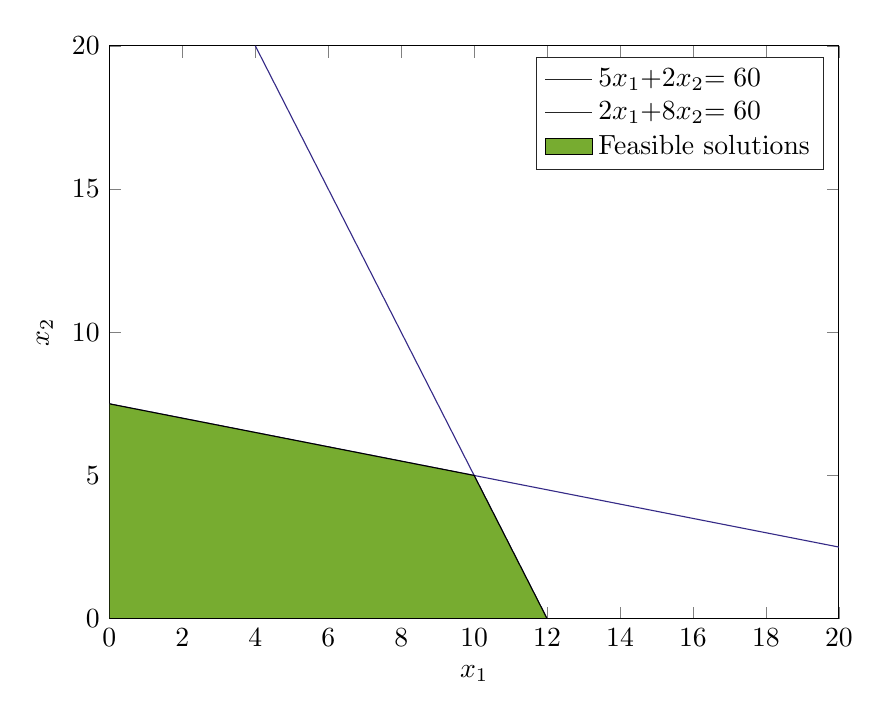
\begin{tikzpicture}

\begin{axis}[%
width=0.764\textwidth,
height=0.6\textwidth,
at={(0\textwidth,0\textwidth)},
scale only axis,
colormap={mymap}{[1pt] rgb(0pt)=(0.2081,0.1663,0.5292); rgb(1pt)=(0.211624,0.189781,0.577676); rgb(2pt)=(0.212252,0.213771,0.626971); rgb(3pt)=(0.2081,0.2386,0.677086); rgb(4pt)=(0.195905,0.264457,0.7279); rgb(5pt)=(0.170729,0.291938,0.779248); rgb(6pt)=(0.125271,0.324243,0.830271); rgb(7pt)=(0.0591333,0.359833,0.868333); rgb(8pt)=(0.0116952,0.38751,0.881957); rgb(9pt)=(0.00595714,0.408614,0.882843); rgb(10pt)=(0.0165143,0.4266,0.878633); rgb(11pt)=(0.0328524,0.443043,0.871957); rgb(12pt)=(0.0498143,0.458571,0.864057); rgb(13pt)=(0.0629333,0.47369,0.855438); rgb(14pt)=(0.0722667,0.488667,0.8467); rgb(15pt)=(0.0779429,0.503986,0.838371); rgb(16pt)=(0.0793476,0.520024,0.831181); rgb(17pt)=(0.0749429,0.537543,0.826271); rgb(18pt)=(0.0640571,0.556986,0.823957); rgb(19pt)=(0.0487714,0.577224,0.822829); rgb(20pt)=(0.0343429,0.596581,0.819852); rgb(21pt)=(0.0265,0.6137,0.8135); rgb(22pt)=(0.0238905,0.628662,0.803762); rgb(23pt)=(0.0230905,0.641786,0.791267); rgb(24pt)=(0.0227714,0.653486,0.776757); rgb(25pt)=(0.0266619,0.664195,0.760719); rgb(26pt)=(0.0383714,0.674271,0.743552); rgb(27pt)=(0.0589714,0.683757,0.725386); rgb(28pt)=(0.0843,0.692833,0.706167); rgb(29pt)=(0.113295,0.7015,0.685857); rgb(30pt)=(0.145271,0.709757,0.664629); rgb(31pt)=(0.180133,0.717657,0.642433); rgb(32pt)=(0.217829,0.725043,0.619262); rgb(33pt)=(0.258643,0.731714,0.595429); rgb(34pt)=(0.302171,0.737605,0.571186); rgb(35pt)=(0.348167,0.742433,0.547267); rgb(36pt)=(0.395257,0.7459,0.524443); rgb(37pt)=(0.44201,0.748081,0.503314); rgb(38pt)=(0.487124,0.749062,0.483976); rgb(39pt)=(0.530029,0.749114,0.466114); rgb(40pt)=(0.570857,0.748519,0.44939); rgb(41pt)=(0.609852,0.747314,0.433686); rgb(42pt)=(0.6473,0.7456,0.4188); rgb(43pt)=(0.683419,0.743476,0.404433); rgb(44pt)=(0.71841,0.741133,0.390476); rgb(45pt)=(0.752486,0.7384,0.376814); rgb(46pt)=(0.785843,0.735567,0.363271); rgb(47pt)=(0.818505,0.732733,0.34979); rgb(48pt)=(0.850657,0.7299,0.336029); rgb(49pt)=(0.882433,0.727433,0.3217); rgb(50pt)=(0.913933,0.725786,0.306276); rgb(51pt)=(0.944957,0.726114,0.288643); rgb(52pt)=(0.973895,0.731395,0.266648); rgb(53pt)=(0.993771,0.745457,0.240348); rgb(54pt)=(0.999043,0.765314,0.216414); rgb(55pt)=(0.995533,0.786057,0.196652); rgb(56pt)=(0.988,0.8066,0.179367); rgb(57pt)=(0.978857,0.827143,0.163314); rgb(58pt)=(0.9697,0.848138,0.147452); rgb(59pt)=(0.962586,0.870514,0.1309); rgb(60pt)=(0.958871,0.8949,0.113243); rgb(61pt)=(0.959824,0.921833,0.0948381); rgb(62pt)=(0.9661,0.951443,0.0755333); rgb(63pt)=(0.9763,0.9831,0.0538)},
xmin=0,
xmax=20,
xlabel={$\text{x}_\text{1}$},
ymin=0,
ymax=20,
ylabel={$\text{x}_\text{2}$},
axis background/.style={fill=white},
legend style={legend cell align=left,align=left,draw=white!15!black}
]
\addplot[contour prepared, contour prepared format=matlab, contour/labels=false] table[row sep=crcr] {%
%
0	351\\
4	20\\
4	20\\
4.032	19.92\\
4.064	19.84\\
4.08	19.8\\
4.096	19.76\\
4.128	19.68\\
4.16	19.6\\
4.16	19.6\\
4.192	19.52\\
4.224	19.44\\
4.24	19.4\\
4.256	19.36\\
4.288	19.28\\
4.32	19.2\\
4.32	19.2\\
4.352	19.12\\
4.384	19.04\\
4.4	19\\
4.416	18.96\\
4.448	18.88\\
4.48	18.8\\
4.48	18.8\\
4.512	18.72\\
4.544	18.64\\
4.56	18.6\\
4.576	18.56\\
4.608	18.48\\
4.64	18.4\\
4.64	18.4\\
4.672	18.32\\
4.704	18.24\\
4.72	18.2\\
4.736	18.16\\
4.768	18.08\\
4.8	18\\
4.8	18\\
4.832	17.92\\
4.864	17.84\\
4.88	17.8\\
4.896	17.76\\
4.928	17.68\\
4.96	17.6\\
4.96	17.6\\
4.992	17.52\\
5.024	17.44\\
5.04	17.4\\
5.056	17.36\\
5.088	17.28\\
5.12	17.2\\
5.12	17.2\\
5.152	17.12\\
5.184	17.04\\
5.2	17\\
5.216	16.96\\
5.248	16.88\\
5.28	16.8\\
5.28	16.8\\
5.312	16.72\\
5.344	16.64\\
5.36	16.6\\
5.376	16.56\\
5.408	16.48\\
5.44	16.4\\
5.44	16.4\\
5.472	16.32\\
5.504	16.24\\
5.52	16.2\\
5.536	16.16\\
5.568	16.08\\
5.6	16\\
5.6	16\\
5.632	15.92\\
5.664	15.84\\
5.68	15.8\\
5.696	15.76\\
5.728	15.68\\
5.76	15.6\\
5.76	15.6\\
5.792	15.52\\
5.824	15.44\\
5.84	15.4\\
5.856	15.36\\
5.888	15.28\\
5.92	15.2\\
5.92	15.2\\
5.952	15.12\\
5.984	15.04\\
6	15\\
6.016	14.96\\
6.048	14.88\\
6.08	14.8\\
6.08	14.8\\
6.112	14.72\\
6.144	14.64\\
6.16	14.6\\
6.176	14.56\\
6.208	14.48\\
6.24	14.4\\
6.24	14.4\\
6.272	14.32\\
6.304	14.24\\
6.32	14.2\\
6.336	14.16\\
6.368	14.08\\
6.4	14\\
6.4	14\\
6.432	13.92\\
6.464	13.84\\
6.48	13.8\\
6.496	13.76\\
6.528	13.68\\
6.56	13.6\\
6.56	13.6\\
6.592	13.52\\
6.624	13.44\\
6.64	13.4\\
6.656	13.36\\
6.688	13.28\\
6.72	13.2\\
6.72	13.2\\
6.752	13.12\\
6.784	13.04\\
6.8	13\\
6.816	12.96\\
6.848	12.88\\
6.88	12.8\\
6.88	12.8\\
6.912	12.72\\
6.944	12.64\\
6.96	12.6\\
6.976	12.56\\
7.008	12.48\\
7.04	12.4\\
7.04	12.4\\
7.072	12.32\\
7.104	12.24\\
7.12	12.2\\
7.136	12.16\\
7.168	12.08\\
7.2	12\\
7.2	12\\
7.232	11.92\\
7.264	11.84\\
7.28	11.8\\
7.296	11.76\\
7.328	11.68\\
7.36	11.6\\
7.36	11.6\\
7.392	11.52\\
7.424	11.44\\
7.44	11.4\\
7.456	11.36\\
7.488	11.28\\
7.52	11.2\\
7.52	11.2\\
7.552	11.12\\
7.584	11.04\\
7.6	11\\
7.616	10.96\\
7.648	10.88\\
7.68	10.8\\
7.68	10.8\\
7.712	10.72\\
7.744	10.64\\
7.76	10.6\\
7.776	10.56\\
7.808	10.48\\
7.84	10.4\\
7.84	10.4\\
7.872	10.32\\
7.904	10.24\\
7.92	10.2\\
7.936	10.16\\
7.968	10.08\\
8	10\\
8	10\\
8.032	9.92\\
8.064	9.84\\
8.08	9.8\\
8.096	9.76\\
8.128	9.68\\
8.16	9.6\\
8.16	9.6\\
8.192	9.52\\
8.224	9.44\\
8.24	9.4\\
8.256	9.36\\
8.288	9.28\\
8.32	9.2\\
8.32	9.2\\
8.352	9.12\\
8.384	9.04\\
8.4	9\\
8.416	8.96\\
8.448	8.88\\
8.48	8.8\\
8.48	8.8\\
8.512	8.72\\
8.544	8.64\\
8.56	8.6\\
8.576	8.56\\
8.608	8.48\\
8.64	8.4\\
8.64	8.4\\
8.672	8.32\\
8.704	8.24\\
8.72	8.2\\
8.736	8.16\\
8.768	8.08\\
8.8	8\\
8.8	8\\
8.832	7.92\\
8.864	7.84\\
8.88	7.8\\
8.896	7.76\\
8.928	7.68\\
8.96	7.6\\
8.96	7.6\\
8.992	7.52\\
9.024	7.44\\
9.04	7.4\\
9.056	7.36\\
9.088	7.28\\
9.12	7.2\\
9.12	7.2\\
9.152	7.12\\
9.184	7.04\\
9.2	7\\
9.216	6.96\\
9.248	6.88\\
9.28	6.8\\
9.28	6.8\\
9.312	6.72\\
9.344	6.64\\
9.36	6.6\\
9.376	6.56\\
9.408	6.48\\
9.44	6.4\\
9.44	6.4\\
9.472	6.32\\
9.504	6.24\\
9.52	6.2\\
9.536	6.16\\
9.568	6.08\\
9.6	6\\
9.6	6\\
9.632	5.92\\
9.664	5.84\\
9.68	5.8\\
9.696	5.76\\
9.728	5.68\\
9.76	5.6\\
9.76	5.6\\
9.792	5.52\\
9.824	5.44\\
9.84	5.4\\
9.856	5.36\\
9.888	5.28\\
9.92	5.2\\
9.92	5.2\\
9.952	5.12\\
9.984	5.04\\
10	5\\
10.016	4.96\\
10.048	4.88\\
10.08	4.8\\
10.08	4.8\\
10.112	4.72\\
10.144	4.64\\
10.16	4.6\\
10.176	4.56\\
10.208	4.48\\
10.24	4.4\\
10.24	4.4\\
10.272	4.32\\
10.304	4.24\\
10.32	4.2\\
10.336	4.16\\
10.368	4.08\\
10.4	4\\
10.4	4\\
10.432	3.92\\
10.464	3.84\\
10.48	3.8\\
10.496	3.76\\
10.528	3.68\\
10.56	3.6\\
10.56	3.6\\
10.592	3.52\\
10.624	3.44\\
10.64	3.4\\
10.656	3.36\\
10.688	3.28\\
10.72	3.2\\
10.72	3.2\\
10.752	3.12\\
10.784	3.04\\
10.8	3\\
10.816	2.96\\
10.848	2.88\\
10.88	2.8\\
10.88	2.8\\
10.912	2.72\\
10.944	2.64\\
10.96	2.6\\
10.976	2.56\\
11.008	2.48\\
11.04	2.4\\
11.04	2.4\\
11.072	2.32\\
11.104	2.24\\
11.12	2.2\\
11.136	2.16\\
11.168	2.08\\
11.2	2\\
11.2	2\\
11.232	1.92\\
11.264	1.84\\
11.28	1.8\\
11.296	1.76\\
11.328	1.68\\
11.36	1.6\\
11.36	1.6\\
11.392	1.52\\
11.424	1.44\\
11.44	1.4\\
11.456	1.36\\
11.488	1.28\\
11.52	1.2\\
11.52	1.2\\
11.552	1.12\\
11.584	1.04\\
11.6	1\\
11.616	0.96\\
11.648	0.88\\
11.68	0.8\\
11.68	0.8\\
11.712	0.72\\
11.744	0.64\\
11.76	0.600000000000002\\
11.776	0.56\\
11.808	0.48\\
11.84	0.4\\
11.84	0.4\\
11.872	0.32\\
11.904	0.24\\
11.92	0.2\\
11.936	0.16\\
11.968	0.08\\
12	0\\
};
\addlegendentry{$\text{5x}_\text{1}\text{ + 2x}_\text{2}\text{ = 60}$};

\addplot[contour prepared, contour prepared format=matlab, contour/labels=false] table[row sep=crcr] {%
%
0	313\\
0	7.5\\
0.08	7.48\\
0.16	7.46\\
0.24	7.44\\
0.24	7.44\\
0.32	7.42\\
0.4	7.4\\
0.48	7.38\\
0.56	7.36\\
0.56	7.36\\
0.64	7.34\\
0.72	7.32\\
0.8	7.3\\
0.88	7.28\\
0.88	7.28\\
0.96	7.26\\
1.04	7.24\\
1.12	7.22\\
1.2	7.2\\
1.2	7.2\\
1.28	7.18\\
1.36	7.16\\
1.44	7.14\\
1.52	7.12\\
1.52	7.12\\
1.6	7.1\\
1.68	7.08\\
1.76	7.06\\
1.84	7.04\\
1.84	7.04\\
1.92	7.02\\
2	7\\
2.08	6.98\\
2.16	6.96\\
2.16	6.96\\
2.24	6.94\\
2.32	6.92\\
2.4	6.9\\
2.48	6.88\\
2.48	6.88\\
2.56	6.86\\
2.64	6.84\\
2.72	6.82\\
2.8	6.8\\
2.8	6.8\\
2.88	6.78\\
2.96	6.76\\
3.04	6.74\\
3.12	6.72\\
3.12	6.72\\
3.2	6.7\\
3.28	6.68\\
3.36	6.66\\
3.44	6.64\\
3.44	6.64\\
3.52	6.62\\
3.6	6.6\\
3.68	6.58\\
3.76	6.56\\
3.76	6.56\\
3.84	6.54\\
3.92	6.52\\
4	6.5\\
4.08	6.48\\
4.08	6.48\\
4.16	6.46\\
4.24	6.44\\
4.32	6.42\\
4.4	6.4\\
4.4	6.4\\
4.48	6.38\\
4.56	6.36\\
4.64	6.34\\
4.72	6.32\\
4.72	6.32\\
4.8	6.3\\
4.88	6.28\\
4.96	6.26\\
5.04	6.24\\
5.04	6.24\\
5.12	6.22\\
5.2	6.2\\
5.28	6.18\\
5.36	6.16\\
5.36	6.16\\
5.44	6.14\\
5.52	6.12\\
5.6	6.1\\
5.68	6.08\\
5.68	6.08\\
5.76	6.06\\
5.84	6.04\\
5.92	6.02\\
6	6\\
6	6\\
6.08	5.98\\
6.16	5.96\\
6.24	5.94\\
6.32	5.92\\
6.32	5.92\\
6.4	5.9\\
6.48	5.88\\
6.56	5.86\\
6.64	5.84\\
6.64	5.84\\
6.72	5.82\\
6.8	5.8\\
6.88	5.78\\
6.96	5.76\\
6.96	5.76\\
7.04	5.74\\
7.12	5.72\\
7.2	5.7\\
7.28	5.68\\
7.28	5.68\\
7.36	5.66\\
7.44	5.64\\
7.52	5.62\\
7.6	5.6\\
7.6	5.6\\
7.68	5.58\\
7.76	5.56\\
7.84	5.54\\
7.92	5.52\\
7.92	5.52\\
8	5.5\\
8.08	5.48\\
8.16	5.46\\
8.24	5.44\\
8.24	5.44\\
8.32	5.42\\
8.4	5.4\\
8.48	5.38\\
8.56	5.36\\
8.56	5.36\\
8.64	5.34\\
8.72	5.32\\
8.8	5.3\\
8.88	5.28\\
8.88	5.28\\
8.96	5.26\\
9.04	5.24\\
9.12	5.22\\
9.2	5.2\\
9.2	5.2\\
9.28	5.18\\
9.36	5.16\\
9.44	5.14\\
9.52	5.12\\
9.52	5.12\\
9.6	5.1\\
9.68	5.08\\
9.76	5.06\\
9.84	5.04\\
9.84	5.04\\
9.92	5.02\\
10	5\\
10.08	4.98\\
10.16	4.96\\
10.16	4.96\\
10.24	4.94\\
10.32	4.92\\
10.4	4.9\\
10.48	4.88\\
10.48	4.88\\
10.56	4.86\\
10.64	4.84\\
10.72	4.82\\
10.8	4.8\\
10.8	4.8\\
10.88	4.78\\
10.96	4.76\\
11.04	4.74\\
11.12	4.72\\
11.12	4.72\\
11.2	4.7\\
11.28	4.68\\
11.36	4.66\\
11.44	4.64\\
11.44	4.64\\
11.52	4.62\\
11.6	4.6\\
11.68	4.58\\
11.76	4.56\\
11.76	4.56\\
11.84	4.54\\
11.92	4.52\\
12	4.5\\
12.08	4.48\\
12.08	4.48\\
12.16	4.46\\
12.24	4.44\\
12.32	4.42\\
12.4	4.4\\
12.4	4.4\\
12.48	4.38\\
12.56	4.36\\
12.64	4.34\\
12.72	4.32\\
12.72	4.32\\
12.8	4.3\\
12.88	4.28\\
12.96	4.26\\
13.04	4.24\\
13.04	4.24\\
13.12	4.22\\
13.2	4.2\\
13.28	4.18\\
13.36	4.16\\
13.36	4.16\\
13.44	4.14\\
13.52	4.12\\
13.6	4.1\\
13.68	4.08\\
13.68	4.08\\
13.76	4.06\\
13.84	4.04\\
13.92	4.02\\
14	4\\
14	4\\
14.08	3.98\\
14.16	3.96\\
14.24	3.94\\
14.32	3.92\\
14.32	3.92\\
14.4	3.9\\
14.48	3.88\\
14.56	3.86\\
14.64	3.84\\
14.64	3.84\\
14.72	3.82\\
14.8	3.8\\
14.88	3.78\\
14.96	3.76\\
14.96	3.76\\
15.04	3.74\\
15.12	3.72\\
15.2	3.7\\
15.28	3.68\\
15.28	3.68\\
15.36	3.66\\
15.44	3.64\\
15.52	3.62\\
15.6	3.6\\
15.6	3.6\\
15.68	3.58\\
15.76	3.56\\
15.84	3.54\\
15.92	3.52\\
15.92	3.52\\
16	3.5\\
16.08	3.48\\
16.16	3.46\\
16.24	3.44\\
16.24	3.44\\
16.32	3.42\\
16.4	3.4\\
16.48	3.38\\
16.56	3.36\\
16.56	3.36\\
16.64	3.34\\
16.72	3.32\\
16.8	3.3\\
16.88	3.28\\
16.88	3.28\\
16.96	3.26\\
17.04	3.24\\
17.12	3.22\\
17.2	3.2\\
17.2	3.2\\
17.28	3.18\\
17.36	3.16\\
17.44	3.14\\
17.52	3.12\\
17.52	3.12\\
17.6	3.1\\
17.68	3.08\\
17.76	3.06\\
17.84	3.04\\
17.84	3.04\\
17.92	3.02\\
18	3\\
18.08	2.98\\
18.16	2.96\\
18.16	2.96\\
18.24	2.94\\
18.32	2.92\\
18.4	2.9\\
18.48	2.88\\
18.48	2.88\\
18.56	2.86\\
18.64	2.84\\
18.72	2.82\\
18.8	2.8\\
18.8	2.8\\
18.88	2.78\\
18.96	2.76\\
19.04	2.74\\
19.12	2.72\\
19.12	2.72\\
19.2	2.7\\
19.28	2.68\\
19.36	2.66\\
19.44	2.64\\
19.44	2.64\\
19.52	2.62\\
19.6	2.6\\
19.68	2.58\\
19.76	2.56\\
19.76	2.56\\
19.84	2.54\\
19.92	2.52\\
20	2.5\\
};
\addlegendentry{$\text{2x}_\text{1}\text{ + 8x}_\text{2}\text{ = 60}$};


\addplot[area legend,solid,draw=black,fill=mycolor1]
table[row sep=crcr] {%
x	y\\
0	7.5\\
10	5\\
12	0\\
0	0\\
}--cycle;
\addlegendentry{Feasible solutions};

\end{axis}
\end{tikzpicture}%
\end{frame}

\begin{frame}
  \frametitle{Plotting the constraints}
  \centering
  % This file was created by matlab2tikz.
%
%The latest updates can be retrieved from
%  http://www.mathworks.com/matlabcentral/fileexchange/22022-matlab2tikz-matlab2tikz
%where you can also make suggestions and rate matlab2tikz.
%
\definecolor{mycolor1}{rgb}{0.46600,0.67400,0.18800}%
%
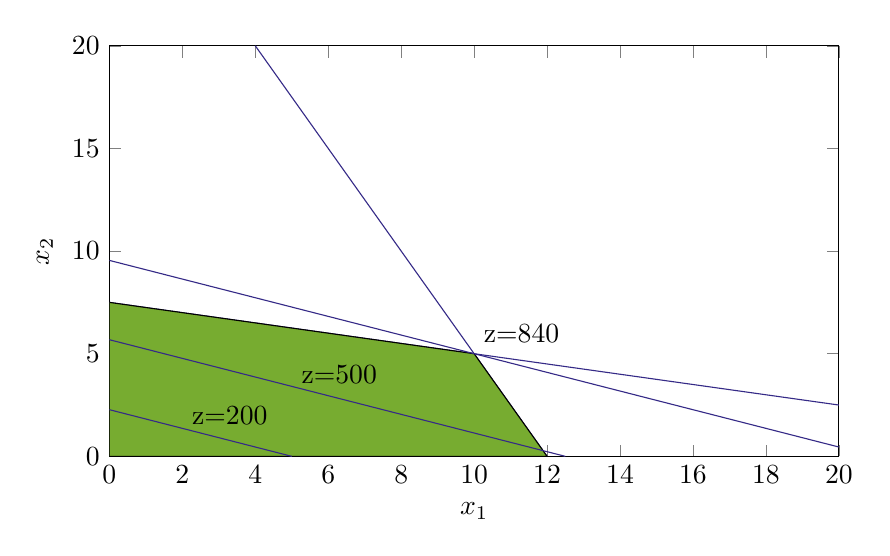
\begin{tikzpicture}

\begin{axis}[%
width=0.764\textwidth,
height=0.43\textwidth,
at={(0\textwidth,0\textwidth)},
scale only axis,
colormap={mymap}{[1pt] rgb(0pt)=(0.2081,0.1663,0.5292); rgb(1pt)=(0.211624,0.189781,0.577676); rgb(2pt)=(0.212252,0.213771,0.626971); rgb(3pt)=(0.2081,0.2386,0.677086); rgb(4pt)=(0.195905,0.264457,0.7279); rgb(5pt)=(0.170729,0.291938,0.779248); rgb(6pt)=(0.125271,0.324243,0.830271); rgb(7pt)=(0.0591333,0.359833,0.868333); rgb(8pt)=(0.0116952,0.38751,0.881957); rgb(9pt)=(0.00595714,0.408614,0.882843); rgb(10pt)=(0.0165143,0.4266,0.878633); rgb(11pt)=(0.0328524,0.443043,0.871957); rgb(12pt)=(0.0498143,0.458571,0.864057); rgb(13pt)=(0.0629333,0.47369,0.855438); rgb(14pt)=(0.0722667,0.488667,0.8467); rgb(15pt)=(0.0779429,0.503986,0.838371); rgb(16pt)=(0.0793476,0.520024,0.831181); rgb(17pt)=(0.0749429,0.537543,0.826271); rgb(18pt)=(0.0640571,0.556986,0.823957); rgb(19pt)=(0.0487714,0.577224,0.822829); rgb(20pt)=(0.0343429,0.596581,0.819852); rgb(21pt)=(0.0265,0.6137,0.8135); rgb(22pt)=(0.0238905,0.628662,0.803762); rgb(23pt)=(0.0230905,0.641786,0.791267); rgb(24pt)=(0.0227714,0.653486,0.776757); rgb(25pt)=(0.0266619,0.664195,0.760719); rgb(26pt)=(0.0383714,0.674271,0.743552); rgb(27pt)=(0.0589714,0.683757,0.725386); rgb(28pt)=(0.0843,0.692833,0.706167); rgb(29pt)=(0.113295,0.7015,0.685857); rgb(30pt)=(0.145271,0.709757,0.664629); rgb(31pt)=(0.180133,0.717657,0.642433); rgb(32pt)=(0.217829,0.725043,0.619262); rgb(33pt)=(0.258643,0.731714,0.595429); rgb(34pt)=(0.302171,0.737605,0.571186); rgb(35pt)=(0.348167,0.742433,0.547267); rgb(36pt)=(0.395257,0.7459,0.524443); rgb(37pt)=(0.44201,0.748081,0.503314); rgb(38pt)=(0.487124,0.749062,0.483976); rgb(39pt)=(0.530029,0.749114,0.466114); rgb(40pt)=(0.570857,0.748519,0.44939); rgb(41pt)=(0.609852,0.747314,0.433686); rgb(42pt)=(0.6473,0.7456,0.4188); rgb(43pt)=(0.683419,0.743476,0.404433); rgb(44pt)=(0.71841,0.741133,0.390476); rgb(45pt)=(0.752486,0.7384,0.376814); rgb(46pt)=(0.785843,0.735567,0.363271); rgb(47pt)=(0.818505,0.732733,0.34979); rgb(48pt)=(0.850657,0.7299,0.336029); rgb(49pt)=(0.882433,0.727433,0.3217); rgb(50pt)=(0.913933,0.725786,0.306276); rgb(51pt)=(0.944957,0.726114,0.288643); rgb(52pt)=(0.973895,0.731395,0.266648); rgb(53pt)=(0.993771,0.745457,0.240348); rgb(54pt)=(0.999043,0.765314,0.216414); rgb(55pt)=(0.995533,0.786057,0.196652); rgb(56pt)=(0.988,0.8066,0.179367); rgb(57pt)=(0.978857,0.827143,0.163314); rgb(58pt)=(0.9697,0.848138,0.147452); rgb(59pt)=(0.962586,0.870514,0.1309); rgb(60pt)=(0.958871,0.8949,0.113243); rgb(61pt)=(0.959824,0.921833,0.0948381); rgb(62pt)=(0.9661,0.951443,0.0755333); rgb(63pt)=(0.9763,0.9831,0.0538)},
xmin=0,
xmax=20,
xlabel={${\text{x}}_{\text{1}}$},
ymin=0,
ymax=20,
ylabel={${\text{x}}_{\text{2}}$},
axis background/.style={fill=white}
]
\addplot[contour prepared, contour prepared format=matlab, contour/labels=false] table[row sep=crcr] {%
%
0	351\\
4	20\\
4	20\\
4.032	19.92\\
4.064	19.84\\
4.08	19.8\\
4.096	19.76\\
4.128	19.68\\
4.16	19.6\\
4.16	19.6\\
4.192	19.52\\
4.224	19.44\\
4.24	19.4\\
4.256	19.36\\
4.288	19.28\\
4.32	19.2\\
4.32	19.2\\
4.352	19.12\\
4.384	19.04\\
4.4	19\\
4.416	18.96\\
4.448	18.88\\
4.48	18.8\\
4.48	18.8\\
4.512	18.72\\
4.544	18.64\\
4.56	18.6\\
4.576	18.56\\
4.608	18.48\\
4.64	18.4\\
4.64	18.4\\
4.672	18.32\\
4.704	18.24\\
4.72	18.2\\
4.736	18.16\\
4.768	18.08\\
4.8	18\\
4.8	18\\
4.832	17.92\\
4.864	17.84\\
4.88	17.8\\
4.896	17.76\\
4.928	17.68\\
4.96	17.6\\
4.96	17.6\\
4.992	17.52\\
5.024	17.44\\
5.04	17.4\\
5.056	17.36\\
5.088	17.28\\
5.12	17.2\\
5.12	17.2\\
5.152	17.12\\
5.184	17.04\\
5.2	17\\
5.216	16.96\\
5.248	16.88\\
5.28	16.8\\
5.28	16.8\\
5.312	16.72\\
5.344	16.64\\
5.36	16.6\\
5.376	16.56\\
5.408	16.48\\
5.44	16.4\\
5.44	16.4\\
5.472	16.32\\
5.504	16.24\\
5.52	16.2\\
5.536	16.16\\
5.568	16.08\\
5.6	16\\
5.6	16\\
5.632	15.92\\
5.664	15.84\\
5.68	15.8\\
5.696	15.76\\
5.728	15.68\\
5.76	15.6\\
5.76	15.6\\
5.792	15.52\\
5.824	15.44\\
5.84	15.4\\
5.856	15.36\\
5.888	15.28\\
5.92	15.2\\
5.92	15.2\\
5.952	15.12\\
5.984	15.04\\
6	15\\
6.016	14.96\\
6.048	14.88\\
6.08	14.8\\
6.08	14.8\\
6.112	14.72\\
6.144	14.64\\
6.16	14.6\\
6.176	14.56\\
6.208	14.48\\
6.24	14.4\\
6.24	14.4\\
6.272	14.32\\
6.304	14.24\\
6.32	14.2\\
6.336	14.16\\
6.368	14.08\\
6.4	14\\
6.4	14\\
6.432	13.92\\
6.464	13.84\\
6.48	13.8\\
6.496	13.76\\
6.528	13.68\\
6.56	13.6\\
6.56	13.6\\
6.592	13.52\\
6.624	13.44\\
6.64	13.4\\
6.656	13.36\\
6.688	13.28\\
6.72	13.2\\
6.72	13.2\\
6.752	13.12\\
6.784	13.04\\
6.8	13\\
6.816	12.96\\
6.848	12.88\\
6.88	12.8\\
6.88	12.8\\
6.912	12.72\\
6.944	12.64\\
6.96	12.6\\
6.976	12.56\\
7.008	12.48\\
7.04	12.4\\
7.04	12.4\\
7.072	12.32\\
7.104	12.24\\
7.12	12.2\\
7.136	12.16\\
7.168	12.08\\
7.2	12\\
7.2	12\\
7.232	11.92\\
7.264	11.84\\
7.28	11.8\\
7.296	11.76\\
7.328	11.68\\
7.36	11.6\\
7.36	11.6\\
7.392	11.52\\
7.424	11.44\\
7.44	11.4\\
7.456	11.36\\
7.488	11.28\\
7.52	11.2\\
7.52	11.2\\
7.552	11.12\\
7.584	11.04\\
7.6	11\\
7.616	10.96\\
7.648	10.88\\
7.68	10.8\\
7.68	10.8\\
7.712	10.72\\
7.744	10.64\\
7.76	10.6\\
7.776	10.56\\
7.808	10.48\\
7.84	10.4\\
7.84	10.4\\
7.872	10.32\\
7.904	10.24\\
7.92	10.2\\
7.936	10.16\\
7.968	10.08\\
8	10\\
8	10\\
8.032	9.92\\
8.064	9.84\\
8.08	9.8\\
8.096	9.76\\
8.128	9.68\\
8.16	9.6\\
8.16	9.6\\
8.192	9.52\\
8.224	9.44\\
8.24	9.4\\
8.256	9.36\\
8.288	9.28\\
8.32	9.2\\
8.32	9.2\\
8.352	9.12\\
8.384	9.04\\
8.4	9\\
8.416	8.96\\
8.448	8.88\\
8.48	8.8\\
8.48	8.8\\
8.512	8.72\\
8.544	8.64\\
8.56	8.6\\
8.576	8.56\\
8.608	8.48\\
8.64	8.4\\
8.64	8.4\\
8.672	8.32\\
8.704	8.24\\
8.72	8.2\\
8.736	8.16\\
8.768	8.08\\
8.8	8\\
8.8	8\\
8.832	7.92\\
8.864	7.84\\
8.88	7.8\\
8.896	7.76\\
8.928	7.68\\
8.96	7.6\\
8.96	7.6\\
8.992	7.52\\
9.024	7.44\\
9.04	7.4\\
9.056	7.36\\
9.088	7.28\\
9.12	7.2\\
9.12	7.2\\
9.152	7.12\\
9.184	7.04\\
9.2	7\\
9.216	6.96\\
9.248	6.88\\
9.28	6.8\\
9.28	6.8\\
9.312	6.72\\
9.344	6.64\\
9.36	6.6\\
9.376	6.56\\
9.408	6.48\\
9.44	6.4\\
9.44	6.4\\
9.472	6.32\\
9.504	6.24\\
9.52	6.2\\
9.536	6.16\\
9.568	6.08\\
9.6	6\\
9.6	6\\
9.632	5.92\\
9.664	5.84\\
9.68	5.8\\
9.696	5.76\\
9.728	5.68\\
9.76	5.6\\
9.76	5.6\\
9.792	5.52\\
9.824	5.44\\
9.84	5.4\\
9.856	5.36\\
9.888	5.28\\
9.92	5.2\\
9.92	5.2\\
9.952	5.12\\
9.984	5.04\\
10	5\\
10.016	4.96\\
10.048	4.88\\
10.08	4.8\\
10.08	4.8\\
10.112	4.72\\
10.144	4.64\\
10.16	4.6\\
10.176	4.56\\
10.208	4.48\\
10.24	4.4\\
10.24	4.4\\
10.272	4.32\\
10.304	4.24\\
10.32	4.2\\
10.336	4.16\\
10.368	4.08\\
10.4	4\\
10.4	4\\
10.432	3.92\\
10.464	3.84\\
10.48	3.8\\
10.496	3.76\\
10.528	3.68\\
10.56	3.6\\
10.56	3.6\\
10.592	3.52\\
10.624	3.44\\
10.64	3.4\\
10.656	3.36\\
10.688	3.28\\
10.72	3.2\\
10.72	3.2\\
10.752	3.12\\
10.784	3.04\\
10.8	3\\
10.816	2.96\\
10.848	2.88\\
10.88	2.8\\
10.88	2.8\\
10.912	2.72\\
10.944	2.64\\
10.96	2.6\\
10.976	2.56\\
11.008	2.48\\
11.04	2.4\\
11.04	2.4\\
11.072	2.32\\
11.104	2.24\\
11.12	2.2\\
11.136	2.16\\
11.168	2.08\\
11.2	2\\
11.2	2\\
11.232	1.92\\
11.264	1.84\\
11.28	1.8\\
11.296	1.76\\
11.328	1.68\\
11.36	1.6\\
11.36	1.6\\
11.392	1.52\\
11.424	1.44\\
11.44	1.4\\
11.456	1.36\\
11.488	1.28\\
11.52	1.2\\
11.52	1.2\\
11.552	1.12\\
11.584	1.04\\
11.6	1\\
11.616	0.96\\
11.648	0.88\\
11.68	0.8\\
11.68	0.8\\
11.712	0.72\\
11.744	0.64\\
11.76	0.600000000000002\\
11.776	0.56\\
11.808	0.48\\
11.84	0.4\\
11.84	0.4\\
11.872	0.32\\
11.904	0.24\\
11.92	0.2\\
11.936	0.16\\
11.968	0.08\\
12	0\\
};
\addplot[contour prepared, contour prepared format=matlab, contour/labels=false] table[row sep=crcr] {%
%
0	313\\
0	7.5\\
0.08	7.48\\
0.16	7.46\\
0.24	7.44\\
0.24	7.44\\
0.32	7.42\\
0.4	7.4\\
0.48	7.38\\
0.56	7.36\\
0.56	7.36\\
0.64	7.34\\
0.72	7.32\\
0.8	7.3\\
0.88	7.28\\
0.88	7.28\\
0.96	7.26\\
1.04	7.24\\
1.12	7.22\\
1.2	7.2\\
1.2	7.2\\
1.28	7.18\\
1.36	7.16\\
1.44	7.14\\
1.52	7.12\\
1.52	7.12\\
1.6	7.1\\
1.68	7.08\\
1.76	7.06\\
1.84	7.04\\
1.84	7.04\\
1.92	7.02\\
2	7\\
2.08	6.98\\
2.16	6.96\\
2.16	6.96\\
2.24	6.94\\
2.32	6.92\\
2.4	6.9\\
2.48	6.88\\
2.48	6.88\\
2.56	6.86\\
2.64	6.84\\
2.72	6.82\\
2.8	6.8\\
2.8	6.8\\
2.88	6.78\\
2.96	6.76\\
3.04	6.74\\
3.12	6.72\\
3.12	6.72\\
3.2	6.7\\
3.28	6.68\\
3.36	6.66\\
3.44	6.64\\
3.44	6.64\\
3.52	6.62\\
3.6	6.6\\
3.68	6.58\\
3.76	6.56\\
3.76	6.56\\
3.84	6.54\\
3.92	6.52\\
4	6.5\\
4.08	6.48\\
4.08	6.48\\
4.16	6.46\\
4.24	6.44\\
4.32	6.42\\
4.4	6.4\\
4.4	6.4\\
4.48	6.38\\
4.56	6.36\\
4.64	6.34\\
4.72	6.32\\
4.72	6.32\\
4.8	6.3\\
4.88	6.28\\
4.96	6.26\\
5.04	6.24\\
5.04	6.24\\
5.12	6.22\\
5.2	6.2\\
5.28	6.18\\
5.36	6.16\\
5.36	6.16\\
5.44	6.14\\
5.52	6.12\\
5.6	6.1\\
5.68	6.08\\
5.68	6.08\\
5.76	6.06\\
5.84	6.04\\
5.92	6.02\\
6	6\\
6	6\\
6.08	5.98\\
6.16	5.96\\
6.24	5.94\\
6.32	5.92\\
6.32	5.92\\
6.4	5.9\\
6.48	5.88\\
6.56	5.86\\
6.64	5.84\\
6.64	5.84\\
6.72	5.82\\
6.8	5.8\\
6.88	5.78\\
6.96	5.76\\
6.96	5.76\\
7.04	5.74\\
7.12	5.72\\
7.2	5.7\\
7.28	5.68\\
7.28	5.68\\
7.36	5.66\\
7.44	5.64\\
7.52	5.62\\
7.6	5.6\\
7.6	5.6\\
7.68	5.58\\
7.76	5.56\\
7.84	5.54\\
7.92	5.52\\
7.92	5.52\\
8	5.5\\
8.08	5.48\\
8.16	5.46\\
8.24	5.44\\
8.24	5.44\\
8.32	5.42\\
8.4	5.4\\
8.48	5.38\\
8.56	5.36\\
8.56	5.36\\
8.64	5.34\\
8.72	5.32\\
8.8	5.3\\
8.88	5.28\\
8.88	5.28\\
8.96	5.26\\
9.04	5.24\\
9.12	5.22\\
9.2	5.2\\
9.2	5.2\\
9.28	5.18\\
9.36	5.16\\
9.44	5.14\\
9.52	5.12\\
9.52	5.12\\
9.6	5.1\\
9.68	5.08\\
9.76	5.06\\
9.84	5.04\\
9.84	5.04\\
9.92	5.02\\
10	5\\
10.08	4.98\\
10.16	4.96\\
10.16	4.96\\
10.24	4.94\\
10.32	4.92\\
10.4	4.9\\
10.48	4.88\\
10.48	4.88\\
10.56	4.86\\
10.64	4.84\\
10.72	4.82\\
10.8	4.8\\
10.8	4.8\\
10.88	4.78\\
10.96	4.76\\
11.04	4.74\\
11.12	4.72\\
11.12	4.72\\
11.2	4.7\\
11.28	4.68\\
11.36	4.66\\
11.44	4.64\\
11.44	4.64\\
11.52	4.62\\
11.6	4.6\\
11.68	4.58\\
11.76	4.56\\
11.76	4.56\\
11.84	4.54\\
11.92	4.52\\
12	4.5\\
12.08	4.48\\
12.08	4.48\\
12.16	4.46\\
12.24	4.44\\
12.32	4.42\\
12.4	4.4\\
12.4	4.4\\
12.48	4.38\\
12.56	4.36\\
12.64	4.34\\
12.72	4.32\\
12.72	4.32\\
12.8	4.3\\
12.88	4.28\\
12.96	4.26\\
13.04	4.24\\
13.04	4.24\\
13.12	4.22\\
13.2	4.2\\
13.28	4.18\\
13.36	4.16\\
13.36	4.16\\
13.44	4.14\\
13.52	4.12\\
13.6	4.1\\
13.68	4.08\\
13.68	4.08\\
13.76	4.06\\
13.84	4.04\\
13.92	4.02\\
14	4\\
14	4\\
14.08	3.98\\
14.16	3.96\\
14.24	3.94\\
14.32	3.92\\
14.32	3.92\\
14.4	3.9\\
14.48	3.88\\
14.56	3.86\\
14.64	3.84\\
14.64	3.84\\
14.72	3.82\\
14.8	3.8\\
14.88	3.78\\
14.96	3.76\\
14.96	3.76\\
15.04	3.74\\
15.12	3.72\\
15.2	3.7\\
15.28	3.68\\
15.28	3.68\\
15.36	3.66\\
15.44	3.64\\
15.52	3.62\\
15.6	3.6\\
15.6	3.6\\
15.68	3.58\\
15.76	3.56\\
15.84	3.54\\
15.92	3.52\\
15.92	3.52\\
16	3.5\\
16.08	3.48\\
16.16	3.46\\
16.24	3.44\\
16.24	3.44\\
16.32	3.42\\
16.4	3.4\\
16.48	3.38\\
16.56	3.36\\
16.56	3.36\\
16.64	3.34\\
16.72	3.32\\
16.8	3.3\\
16.88	3.28\\
16.88	3.28\\
16.96	3.26\\
17.04	3.24\\
17.12	3.22\\
17.2	3.2\\
17.2	3.2\\
17.28	3.18\\
17.36	3.16\\
17.44	3.14\\
17.52	3.12\\
17.52	3.12\\
17.6	3.1\\
17.68	3.08\\
17.76	3.06\\
17.84	3.04\\
17.84	3.04\\
17.92	3.02\\
18	3\\
18.08	2.98\\
18.16	2.96\\
18.16	2.96\\
18.24	2.94\\
18.32	2.92\\
18.4	2.9\\
18.48	2.88\\
18.48	2.88\\
18.56	2.86\\
18.64	2.84\\
18.72	2.82\\
18.8	2.8\\
18.8	2.8\\
18.88	2.78\\
18.96	2.76\\
19.04	2.74\\
19.12	2.72\\
19.12	2.72\\
19.2	2.7\\
19.28	2.68\\
19.36	2.66\\
19.44	2.64\\
19.44	2.64\\
19.52	2.62\\
19.6	2.6\\
19.68	2.58\\
19.76	2.56\\
19.76	2.56\\
19.84	2.54\\
19.92	2.52\\
20	2.5\\
};

\addplot[area legend,solid,draw=black,fill=mycolor1,forget plot]
table[row sep=crcr] {%
x	y\\
0	7.5\\
10	5\\
12	0\\
0	0\\
}--cycle;
\addplot[contour prepared, contour prepared format=matlab, contour/labels=false] table[row sep=crcr] {%
%
0	92\\
0	2.27272727272727\\
0.0720000000000001	2.24\\
0.08	2.23636363636364\\
0.16	2.2\\
0.24	2.16363636363636\\
0.248	2.16\\
0.32	2.12727272727273\\
0.4	2.09090909090909\\
0.424	2.08\\
0.48	2.05454545454545\\
0.56	2.01818181818182\\
0.6	2\\
0.64	1.98181818181818\\
0.72	1.94545454545455\\
0.776	1.92\\
0.8	1.90909090909091\\
0.88	1.87272727272727\\
0.952	1.84\\
0.96	1.83636363636364\\
1.04	1.8\\
1.12	1.76363636363636\\
1.128	1.76\\
1.2	1.72727272727273\\
1.28	1.69090909090909\\
1.304	1.68\\
1.36	1.65454545454545\\
1.44	1.61818181818182\\
1.48	1.6\\
1.52	1.58181818181818\\
1.6	1.54545454545455\\
1.656	1.52\\
1.68	1.50909090909091\\
1.76	1.47272727272727\\
1.832	1.44\\
1.84	1.43636363636364\\
1.92	1.4\\
2	1.36363636363636\\
2.008	1.36\\
2.08	1.32727272727273\\
2.16	1.29090909090909\\
2.184	1.28\\
2.24	1.25454545454545\\
2.32	1.21818181818182\\
2.36	1.2\\
2.4	1.18181818181818\\
2.48	1.14545454545455\\
2.536	1.12\\
2.56	1.10909090909091\\
2.64	1.07272727272727\\
2.712	1.04\\
2.72	1.03636363636364\\
2.8	1\\
2.88	0.963636363636364\\
2.888	0.96\\
2.96	0.927272727272727\\
3.04	0.890909090909091\\
3.064	0.88\\
3.12	0.854545454545454\\
3.2	0.818181818181818\\
3.24	0.8\\
3.28	0.781818181818182\\
3.36	0.745454545454545\\
3.416	0.72\\
3.44	0.709090909090909\\
3.52	0.672727272727273\\
3.592	0.64\\
3.6	0.636363636363636\\
3.68	0.6\\
3.76	0.563636363636364\\
3.768	0.56\\
3.84	0.527272727272727\\
3.92	0.490909090909091\\
3.944	0.48\\
4	0.454545454545455\\
4.08	0.418181818181818\\
4.12	0.4\\
4.16	0.381818181818182\\
4.24	0.345454545454545\\
4.296	0.32\\
4.32	0.309090909090909\\
4.4	0.272727272727273\\
4.472	0.24\\
4.48	0.236363636363636\\
4.56	0.2\\
4.64	0.163636363636364\\
4.648	0.16\\
4.72	0.127272727272727\\
4.8	0.090909090909091\\
4.824	0.08\\
4.88	0.0545454545454547\\
4.96	0.0181818181818181\\
5	0\\
};
\addplot[contour prepared, contour prepared format=matlab, contour/labels=false] table[row sep=crcr] {%
%
0	229\\
0	5.68181818181818\\
0.00400000000000064	5.68\\
0.08	5.64545454545455\\
0.16	5.60909090909091\\
0.180000000000001	5.6\\
0.24	5.57272727272727\\
0.32	5.53636363636364\\
0.356	5.52\\
0.4	5.5\\
0.48	5.46363636363636\\
0.532	5.44\\
0.56	5.42727272727273\\
0.64	5.39090909090909\\
0.708	5.36\\
0.72	5.35454545454545\\
0.8	5.31818181818182\\
0.88	5.28181818181818\\
0.883999999999999	5.28\\
0.96	5.24545454545455\\
1.04	5.20909090909091\\
1.06	5.2\\
1.12	5.17272727272727\\
1.2	5.13636363636364\\
1.236	5.12\\
1.28	5.1\\
1.36	5.06363636363636\\
1.412	5.04\\
1.44	5.02727272727273\\
1.52	4.99090909090909\\
1.588	4.96\\
1.6	4.95454545454545\\
1.68	4.91818181818182\\
1.76	4.88181818181818\\
1.764	4.88\\
1.84	4.84545454545454\\
1.92	4.80909090909091\\
1.94	4.8\\
2	4.77272727272727\\
2.08	4.73636363636364\\
2.116	4.72\\
2.16	4.7\\
2.24	4.66363636363636\\
2.292	4.64\\
2.32	4.62727272727273\\
2.4	4.59090909090909\\
2.468	4.56\\
2.48	4.55454545454545\\
2.56	4.51818181818182\\
2.64	4.48181818181818\\
2.644	4.48\\
2.72	4.44545454545455\\
2.8	4.40909090909091\\
2.82	4.4\\
2.88	4.37272727272727\\
2.96	4.33636363636364\\
2.996	4.32\\
3.04	4.3\\
3.12	4.26363636363636\\
3.172	4.24\\
3.2	4.22727272727273\\
3.28	4.19090909090909\\
3.348	4.16\\
3.36	4.15454545454545\\
3.44	4.11818181818182\\
3.52	4.08181818181818\\
3.524	4.08\\
3.6	4.04545454545454\\
3.68	4.00909090909091\\
3.7	4\\
3.76	3.97272727272727\\
3.84	3.93636363636364\\
3.876	3.92\\
3.92	3.9\\
4	3.86363636363636\\
4.052	3.84\\
4.08	3.82727272727273\\
4.16	3.79090909090909\\
4.228	3.76\\
4.24	3.75454545454545\\
4.32	3.71818181818182\\
4.4	3.68181818181818\\
4.404	3.68\\
4.48	3.64545454545455\\
4.56	3.60909090909091\\
4.58	3.6\\
4.64	3.57272727272727\\
4.72	3.53636363636364\\
4.756	3.52\\
4.8	3.5\\
4.88	3.46363636363636\\
4.932	3.44\\
4.96	3.42727272727273\\
5.04	3.39090909090909\\
5.108	3.36\\
5.12	3.35454545454545\\
5.2	3.31818181818182\\
5.28	3.28181818181818\\
5.284	3.28\\
5.36	3.24545454545455\\
5.44	3.20909090909091\\
5.46	3.2\\
5.52	3.17272727272727\\
5.6	3.13636363636364\\
5.636	3.12\\
5.68	3.1\\
5.76	3.06363636363636\\
5.812	3.04\\
5.84	3.02727272727273\\
5.92	2.99090909090909\\
5.988	2.96\\
6	2.95454545454545\\
6.08	2.91818181818182\\
6.16	2.88181818181818\\
6.164	2.88\\
6.24	2.84545454545455\\
6.32	2.80909090909091\\
6.34	2.8\\
6.4	2.77272727272727\\
6.48	2.73636363636364\\
6.516	2.72\\
6.56	2.7\\
6.64	2.66363636363636\\
6.692	2.64\\
6.72	2.62727272727273\\
6.8	2.59090909090909\\
6.868	2.56\\
6.88	2.55454545454545\\
6.96	2.51818181818182\\
7.04	2.48181818181818\\
7.044	2.48\\
7.12	2.44545454545455\\
7.2	2.40909090909091\\
7.22	2.4\\
7.28	2.37272727272727\\
7.36	2.33636363636364\\
7.396	2.32\\
7.44	2.3\\
7.52	2.26363636363636\\
7.572	2.24\\
7.6	2.22727272727273\\
7.68	2.19090909090909\\
7.748	2.16\\
7.76	2.15454545454545\\
7.84	2.11818181818182\\
7.92	2.08181818181818\\
7.924	2.08\\
8	2.04545454545455\\
8.08	2.00909090909091\\
8.1	2\\
8.16	1.97272727272727\\
8.24	1.93636363636364\\
8.276	1.92\\
8.32	1.9\\
8.4	1.86363636363636\\
8.452	1.84\\
8.48	1.82727272727273\\
8.56	1.79090909090909\\
8.628	1.76\\
8.64	1.75454545454545\\
8.72	1.71818181818182\\
8.8	1.68181818181818\\
8.804	1.68\\
8.88	1.64545454545454\\
8.96	1.60909090909091\\
8.98	1.6\\
9.04	1.57272727272727\\
9.12	1.53636363636364\\
9.156	1.52\\
9.2	1.5\\
9.28	1.46363636363636\\
9.332	1.44\\
9.36	1.42727272727273\\
9.44	1.39090909090909\\
9.508	1.36\\
9.52	1.35454545454546\\
9.6	1.31818181818182\\
9.68	1.28181818181818\\
9.684	1.28\\
9.76	1.24545454545455\\
9.84	1.20909090909091\\
9.86	1.2\\
9.92	1.17272727272727\\
10	1.13636363636364\\
10.036	1.12\\
10.08	1.1\\
10.16	1.06363636363636\\
10.212	1.04\\
10.24	1.02727272727273\\
10.32	0.990909090909091\\
10.388	0.96\\
10.4	0.954545454545454\\
10.48	0.918181818181818\\
10.56	0.881818181818182\\
10.564	0.88\\
10.64	0.845454545454545\\
10.72	0.809090909090909\\
10.74	0.8\\
10.8	0.772727272727273\\
10.88	0.736363636363636\\
10.916	0.72\\
10.96	0.7\\
11.04	0.663636363636364\\
11.092	0.64\\
11.12	0.627272727272728\\
11.2	0.590909090909091\\
11.268	0.56\\
11.28	0.554545454545454\\
11.36	0.518181818181819\\
11.44	0.481818181818182\\
11.444	0.48\\
11.52	0.445454545454546\\
11.6	0.409090909090909\\
11.62	0.4\\
11.68	0.372727272727273\\
11.76	0.336363636363636\\
11.796	0.32\\
11.84	0.299999999999999\\
11.92	0.263636363636363\\
11.972	0.24\\
12	0.227272727272727\\
12.08	0.190909090909091\\
12.148	0.16\\
12.16	0.154545454545455\\
12.24	0.118181818181818\\
12.32	0.0818181818181815\\
12.324	0.08\\
12.4	0.0454545454545453\\
12.48	0.00909090909090855\\
12.5	0\\
};
\addplot[contour prepared, contour prepared format=matlab, contour/labels=false] table[row sep=crcr] {%
%
0	365\\
0	9.54545454545454\\
0.0559999999999994	9.52\\
0.08	9.50909090909091\\
0.16	9.47272727272727\\
0.232000000000002	9.44\\
0.24	9.43636363636364\\
0.32	9.4\\
0.4	9.36363636363636\\
0.408000000000001	9.36\\
0.48	9.32727272727273\\
0.56	9.29090909090909\\
0.584000000000001	9.28\\
0.64	9.25454545454545\\
0.72	9.21818181818182\\
0.760000000000003	9.2\\
0.8	9.18181818181818\\
0.88	9.14545454545454\\
0.936000000000001	9.12\\
0.96	9.10909090909091\\
1.04	9.07272727272727\\
1.112	9.04\\
1.12	9.03636363636364\\
1.2	9\\
1.28	8.96363636363636\\
1.288	8.96\\
1.36	8.92727272727273\\
1.44	8.89090909090909\\
1.464	8.88\\
1.52	8.85454545454546\\
1.6	8.81818181818182\\
1.64	8.8\\
1.68	8.78181818181818\\
1.76	8.74545454545455\\
1.816	8.72\\
1.84	8.70909090909091\\
1.92	8.67272727272727\\
1.992	8.64\\
2	8.63636363636364\\
2.08	8.6\\
2.16	8.56363636363636\\
2.168	8.56\\
2.24	8.52727272727273\\
2.32	8.49090909090909\\
2.344	8.48\\
2.4	8.45454545454546\\
2.48	8.41818181818182\\
2.52	8.4\\
2.56	8.38181818181818\\
2.64	8.34545454545454\\
2.696	8.32\\
2.72	8.30909090909091\\
2.8	8.27272727272727\\
2.872	8.24\\
2.88	8.23636363636364\\
2.96	8.2\\
3.04	8.16363636363636\\
3.048	8.16\\
3.12	8.12727272727273\\
3.2	8.09090909090909\\
3.224	8.08\\
3.28	8.05454545454545\\
3.36	8.01818181818182\\
3.4	8\\
3.44	7.98181818181818\\
3.52	7.94545454545455\\
3.576	7.92\\
3.6	7.90909090909091\\
3.68	7.87272727272727\\
3.752	7.84\\
3.76	7.83636363636364\\
3.84	7.8\\
3.92	7.76363636363636\\
3.928	7.76\\
4	7.72727272727273\\
4.08	7.69090909090909\\
4.104	7.68\\
4.16	7.65454545454546\\
4.24	7.61818181818182\\
4.28	7.6\\
4.32	7.58181818181818\\
4.4	7.54545454545454\\
4.456	7.52\\
4.48	7.50909090909091\\
4.56	7.47272727272727\\
4.632	7.44\\
4.64	7.43636363636364\\
4.72	7.4\\
4.8	7.36363636363636\\
4.808	7.36\\
4.88	7.32727272727273\\
4.96	7.29090909090909\\
4.984	7.28\\
5.04	7.25454545454545\\
5.12	7.21818181818182\\
5.16	7.2\\
5.2	7.18181818181818\\
5.28	7.14545454545454\\
5.336	7.12\\
5.36	7.10909090909091\\
5.44	7.07272727272727\\
5.512	7.04\\
5.52	7.03636363636364\\
5.6	7\\
5.68	6.96363636363636\\
5.688	6.96\\
5.76	6.92727272727273\\
5.84	6.89090909090909\\
5.864	6.88\\
5.92	6.85454545454545\\
6	6.81818181818182\\
6.04	6.8\\
6.08	6.78181818181818\\
6.16	6.74545454545455\\
6.216	6.72\\
6.24	6.70909090909091\\
6.32	6.67272727272727\\
6.392	6.64\\
6.4	6.63636363636364\\
6.48	6.6\\
6.56	6.56363636363636\\
6.568	6.56\\
6.64	6.52727272727273\\
6.72	6.49090909090909\\
6.744	6.48\\
6.8	6.45454545454546\\
6.88	6.41818181818182\\
6.92	6.4\\
6.96	6.38181818181818\\
7.04	6.34545454545454\\
7.096	6.32\\
7.12	6.30909090909091\\
7.2	6.27272727272727\\
7.272	6.24\\
7.28	6.23636363636364\\
7.36	6.2\\
7.44	6.16363636363636\\
7.448	6.16\\
7.52	6.12727272727273\\
7.6	6.09090909090909\\
7.624	6.08\\
7.68	6.05454545454545\\
7.76	6.01818181818182\\
7.8	6\\
7.84	5.98181818181818\\
7.92	5.94545454545455\\
7.976	5.92\\
8	5.90909090909091\\
8.08	5.87272727272727\\
8.152	5.84\\
8.16	5.83636363636364\\
8.24	5.8\\
8.32	5.76363636363636\\
8.328	5.76\\
8.4	5.72727272727273\\
8.48	5.69090909090909\\
8.504	5.68\\
8.56	5.65454545454545\\
8.64	5.61818181818182\\
8.68	5.6\\
8.72	5.58181818181818\\
8.8	5.54545454545454\\
8.856	5.52\\
8.88	5.50909090909091\\
8.96	5.47272727272727\\
9.032	5.44\\
9.04	5.43636363636364\\
9.12	5.4\\
9.2	5.36363636363636\\
9.208	5.36\\
9.28	5.32727272727273\\
9.36	5.29090909090909\\
9.384	5.28\\
9.44	5.25454545454545\\
9.52	5.21818181818182\\
9.56	5.2\\
9.6	5.18181818181818\\
9.68	5.14545454545455\\
9.736	5.12\\
9.76	5.10909090909091\\
9.84	5.07272727272727\\
9.912	5.04\\
9.92	5.03636363636364\\
10	5\\
10.08	4.96363636363636\\
10.088	4.96\\
10.16	4.92727272727273\\
10.24	4.89090909090909\\
10.264	4.88\\
10.32	4.85454545454545\\
10.4	4.81818181818182\\
10.44	4.8\\
10.48	4.78181818181818\\
10.56	4.74545454545455\\
10.616	4.72\\
10.64	4.70909090909091\\
10.72	4.67272727272727\\
10.792	4.64\\
10.8	4.63636363636364\\
10.88	4.6\\
10.96	4.56363636363636\\
10.968	4.56\\
11.04	4.52727272727273\\
11.12	4.49090909090909\\
11.144	4.48\\
11.2	4.45454545454546\\
11.28	4.41818181818182\\
11.32	4.4\\
11.36	4.38181818181818\\
11.44	4.34545454545455\\
11.496	4.32\\
11.52	4.30909090909091\\
11.6	4.27272727272727\\
11.672	4.24\\
11.68	4.23636363636364\\
11.76	4.2\\
11.84	4.16363636363636\\
11.848	4.16\\
11.92	4.12727272727273\\
12	4.09090909090909\\
12.024	4.08\\
12.08	4.05454545454545\\
12.16	4.01818181818182\\
12.2	4\\
12.24	3.98181818181818\\
12.32	3.94545454545455\\
12.376	3.92\\
12.4	3.90909090909091\\
12.48	3.87272727272727\\
12.552	3.84\\
12.56	3.83636363636364\\
12.64	3.8\\
12.72	3.76363636363636\\
12.728	3.76\\
12.8	3.72727272727273\\
12.88	3.69090909090909\\
12.904	3.68\\
12.96	3.65454545454545\\
13.04	3.61818181818182\\
13.08	3.6\\
13.12	3.58181818181818\\
13.2	3.54545454545455\\
13.256	3.52\\
13.28	3.50909090909091\\
13.36	3.47272727272727\\
13.432	3.44\\
13.44	3.43636363636364\\
13.52	3.4\\
13.6	3.36363636363636\\
13.608	3.36\\
13.68	3.32727272727273\\
13.76	3.29090909090909\\
13.784	3.28\\
13.84	3.25454545454545\\
13.92	3.21818181818182\\
13.96	3.2\\
14	3.18181818181818\\
14.08	3.14545454545455\\
14.136	3.12\\
14.16	3.10909090909091\\
14.24	3.07272727272727\\
14.312	3.04\\
14.32	3.03636363636364\\
14.4	3\\
14.48	2.96363636363636\\
14.488	2.96\\
14.56	2.92727272727273\\
14.64	2.89090909090909\\
14.664	2.88\\
14.72	2.85454545454545\\
14.8	2.81818181818182\\
14.84	2.8\\
14.88	2.78181818181818\\
14.96	2.74545454545454\\
15.016	2.72\\
15.04	2.70909090909091\\
15.12	2.67272727272727\\
15.192	2.64\\
15.2	2.63636363636364\\
15.28	2.6\\
15.36	2.56363636363636\\
15.368	2.56\\
15.44	2.52727272727273\\
15.52	2.49090909090909\\
15.544	2.48\\
15.6	2.45454545454545\\
15.68	2.41818181818182\\
15.72	2.4\\
15.76	2.38181818181818\\
15.84	2.34545454545455\\
15.896	2.32\\
15.92	2.30909090909091\\
16	2.27272727272727\\
16.072	2.24\\
16.08	2.23636363636364\\
16.16	2.2\\
16.24	2.16363636363636\\
16.248	2.16\\
16.32	2.12727272727273\\
16.4	2.09090909090909\\
16.424	2.08\\
16.48	2.05454545454545\\
16.56	2.01818181818182\\
16.6	2\\
16.64	1.98181818181818\\
16.72	1.94545454545455\\
16.776	1.92\\
16.8	1.90909090909091\\
16.88	1.87272727272727\\
16.952	1.84\\
16.96	1.83636363636363\\
17.04	1.8\\
17.12	1.76363636363636\\
17.128	1.76\\
17.2	1.72727272727273\\
17.28	1.69090909090909\\
17.304	1.68\\
17.36	1.65454545454545\\
17.44	1.61818181818182\\
17.48	1.6\\
17.52	1.58181818181818\\
17.6	1.54545454545455\\
17.656	1.52\\
17.68	1.50909090909091\\
17.76	1.47272727272727\\
17.832	1.44\\
17.84	1.43636363636364\\
17.92	1.4\\
18	1.36363636363636\\
18.008	1.36\\
18.08	1.32727272727273\\
18.16	1.29090909090909\\
18.184	1.28\\
18.24	1.25454545454546\\
18.32	1.21818181818182\\
18.36	1.2\\
18.4	1.18181818181818\\
18.48	1.14545454545455\\
18.536	1.12\\
18.56	1.10909090909091\\
18.64	1.07272727272727\\
18.712	1.04\\
18.72	1.03636363636364\\
18.8	1\\
18.88	0.963636363636364\\
18.888	0.96\\
18.96	0.927272727272726\\
19.04	0.890909090909091\\
19.064	0.88\\
19.12	0.854545454545454\\
19.2	0.818181818181818\\
19.24	0.8\\
19.28	0.781818181818182\\
19.36	0.745454545454546\\
19.416	0.72\\
19.44	0.709090909090909\\
19.52	0.672727272727273\\
19.592	0.64\\
19.6	0.636363636363636\\
19.68	0.599999999999999\\
19.76	0.563636363636363\\
19.768	0.56\\
19.84	0.527272727272727\\
19.92	0.49090909090909\\
19.944	0.48\\
20	0.454545454545454\\
};
\node[right, align=left, text=black]
at (axis cs:2,2) {z=200};
\node[right, align=left, text=black]
at (axis cs:5,4) {z=500};
\node[right, align=left, text=black]
at (axis cs:10,6) {z=840};
\end{axis}
\end{tikzpicture}%
\end{frame}

\begin{frame}
  \frametitle{Normal form of an LP problem}
   \begin{columns}[T]
    \column{0.5\textwidth}
      $\max z = f(x_1, x_2)=40x_1 + 88x_2$ \\
      s.t. \\
      $2x_1 + 8x_2 \leq 60$ \\
      $5x_1 + 2x_2 \leq 60$ \\
      $x_1 \geq 0$ \\
      $x_2 \geq 0$
    \pause
    \column{0.5\textwidth}
      $\max z = f(x) = 40x_1 + 88x_2$ \\
      s.t. \\
      $2x_1 + 8x_2 + x_3 = 60$ \\
      $5x_1 + 2x_2 + x_4 = 60$ \\
      $x_i \geq 0 \qquad i \in 1,2,3,4$\\
      \vskip1em
      \tikz{\node[emphblock, text width=\columnwidth]{$x_3$ and $x_4$ are called slack variables, they are non auxiliary variables introduced for the purpose of converting inequalities in to equalities}}
  \end{columns}
  \end{frame}

  \begin{frame}
  \frametitle{The simplex method}
  We can formulate our earlier example to the normal form and consider it as the following augmented matrix with $T_0 = \left[z \quad x_1 \quad x_2 \quad x_3 \quad x_4 \quad b\right]$:
  \vskip1em
   \[
T_0 = \begin{bmatrix}
1 & -40 & -88 & 0 & 0 & 0\\ 
0 & 2 & 8 & 1 & 0 & 60\\
0 & 5 & 2 & 0 & 1 &60 
\end{bmatrix}
   \]
   This matrix is called the (initial) simplex table. Each simplex table has two kinds of variables, the basic variables (columns having only one nonzero entry) and the nonbasic variables
\end{frame}

\begin{frame}
  \frametitle{The simplex method}
     \[
T_0 = \begin{bmatrix}
1 & -40 & -88 & 0 & 0 & 0\\ 
0 & 2 & 8 & 1 & 0 & 60\\
0 & 5 & 2 & 0 & 1 &60 
\end{bmatrix}
   \]
   Every simplex table has a feasible solution. It can be obtained by setting the nonbasic variables to zero: $x_1 = 0$, $x_2 = 0$, $x_3 = 60/1$, $x_4 = 60/1$, $z = 0$.
\end{frame}

\begin{frame}
  \frametitle{The optimal solution?}
  \begin{itemize}
    \item The optimal solution is now obtained stepwise by pivoting in such way that z reaches a maximum. 
    \item The big question is, how to choose your pivot equation ...
  \end{itemize}
\end{frame}

\begin{frame}
  \frametitle{Step 1: Selection of the pivot column}
  Select as the column of the pivot, the first column with a negative entry in Row 1. In our example, that’s column 2 (-40)
     \[
T_0 = \begin{bmatrix}
1 & -40 & -88 & 0 & 0 & 0\\ 
0 & 2 & 8 & 1 & 0 & 60\\
0 & 5 & 2 & 0 & 1 &60 
\end{bmatrix}
   \]
\end{frame}

\begin{frame}
  \frametitle{Step 2: Selection of the pivot row}
  Divide the right sides by the corresponding column entries of the selected pivot column. In our example that is $60/2 = 30$ and $60/5 = 12$.
     \[
T_0 = \begin{bmatrix}
1 & -40 & -88 & 0 & 0 & 0\\ 
0 & 2 & 8 & 1 & 0 & 60\\
0 & 5 & 2 & 0 & 1 &60 
\end{bmatrix}
   \]
   Take as the pivot equation the equation that gives the smallest quotient, so $60/5$.
\end{frame}

\begin{frame}
  \frametitle{Step 3: Elimination by row operations}
  \begin{itemize}
    \item Row 1 = Row 1 + 8 * Row 3
    \item Row 2 = Row 2 - 0.4 * Row 3
  \end{itemize}
     \[
T_1 = \begin{bmatrix}
1 & 0 & -72 & 0 & 8 & 480\\ 
0 & 0 & 7.2 & 1 & -0.4 & 36\\
0 & 5 & 2 & 0 & 1 &60 
\end{bmatrix}
   \]
   The basic variables are now $x_1$, $x_3$ and the nonbasic variables are $x_2$, $x_4$. Setting the nonbasic variables to zero will give a new feasible solution: $x_1 = 60/5$, $x_2 = 0$, $x_3 = 36/1$, $x_4 = 0$, $z =480$.
\end{frame}

\begin{frame}
  \frametitle{The simplex method}
  \begin{itemize}
    \item We moved from z = 0 to z = 480. The reason for the increase is because we eliminated a negative term from the eqation, so: elimination should only be applied to negative entries in Row 1, but no others.
    \item Although we found a feasible solution, we did not find the optimal solution yet (the entry of -72 in our simplex table) $\longrightarrow$ repeat step 1 to 3. 
  \end{itemize}
\end{frame}

\begin{frame}
  \frametitle{The simplex method}
  Another iteration is required:
  \begin{itemize}
    \item Step 1: Select column 3
    \item Step 2: $36/7.2 = 5$ and $60/2 = 30$ $\longrightarrow$ select 7.2 as the pivot
    \item Elimination by row operations:
    \begin{itemize}
      \item Row 1 = Row 1 + 10*Row 2
      \item Row 3 = Row 3 - (2/7.2)*Row 2
    \end{itemize}
       \[
T_2 = \begin{bmatrix}
1 & 0 & 0 & 10 & 4 & 840\\ 
0 & 0 & 7.2 & 1 & -0.4 & 36\\
0 & 5 & 0 & -1/36 & 1/0.9 &50 
\end{bmatrix}
   \]
    \item The basic feasible solution: $x_1 = 50/5$, $x_2 = 36/7.2$, $x_3 = 0$, $x_4 = 0$, $z=840$ (no more negative entries: so this solution is also the optimal solution)
  \end{itemize}
\end{frame}

\begin{frame}[fragile]
  \frametitle{Using Python for LP problems}
  \begin{columns}
    \column{0.5\textwidth}
    We are going to solve the following LP problem:\\
    \[
    \min f(x) = -5x_1 -4x_2 - 6x_3 
    \] 
    s.t. \\
    \[
    \begin{array}{l}
    x_1 - x_2 + x_3 \leq 20 \\
    3x_1 + 2x_2 + 4x_3 \leq 42 \\
    3x_1 + 2x_2 \leq 30 
    \end{array}
    \]
    \[
    \begin{array}{l}
    x_1 \geq 0 \\
    x_2 \geq 0 \\
    x_3 \geq 0
    \end{array}
    \]
    \column{0.5\textwidth}
    Using the function \texttt{linprog} from \texttt{scipy.optimize}:
    \begin{lstlisting}[language=Python, basicstyle=\scriptsize]
from scipy.optimize import linprog

c = [-5, -4, -6]
A = [[1, -1, 1], [3, 2, 4], [3, 2, 0]]
b = [20, 42, 30]
bounds = [(0, None), (0, None), (0, None)]

res = linprog(c, A_ub=A, b_ub=b, bounds=bounds)
    \end{lstlisting}
Gives (after accessing appropriate attributes of the result object):
    \begin{lstlisting}[language=Python, basicstyle=\scriptsize]
x = res.x
fun = res.fun
slack = res.slack
success = res.success
    \end{lstlisting}
  \end{columns}
\end{frame}


% \section{Non-linear programming}
% \begin{frame}
%   \frametitle{Non-linear programming}
%   \begin{itemize}
%     \item In nonlinear programming the objective function and the constraints are nonlinear functions. For example: \vskip1em
%     $\min f(x) = -5x_1^2 + 3x_2^2$ \\
%     s.t. \\
%     $g(x) = 2x_1 + x_2 - 5 = 0$ 
%     \vskip1em \pause
%     \item Using the Lagrange multiplier method, a Lagrangian function can be defined as:
%     \[
%       L(x,v) = f(x) + vg(x)
%     \] \pause
%   \item The optimum is found by differentiation of $L$ with respect to $x$ and $v$ and set the equations to zero:
%   \[
%     \frac{\partial L}{\partial x} = \frac{\partial f}{\partial x} + v\frac{\partial g}{\partial x} = 0, \, g(x) = 0
%   \]
%   \end{itemize}
% \end{frame}
% 
% \begin{frame}
%   \frametitle{Lagrange multiplier method}
%    $\min f(x) = -5x_1^2 + 3x_2^2$ \\
%     s.t. \\
%     $g(x) = 2x_1 + x_2 - 5 = 0$ \\
%     \vskip1em \pause
%     \[
%       L = 5x_1^2 + 3x_2^2 + v(2x_1 + x_2 - 5)
%     \]
%     \pause
%     \[ 
% \left.\begin{matrix}
% \frac{\partial L}{\partial x_1} = 10x_1 + 2v = 0 \\ 
% \frac{\partial L}{\partial x_2} = 6x_2 + v = 0  \\ 
% \frac{\partial L}{\partial v} = g(x) = 2x_1 + x_2 - 5 = 0
% \end{matrix}\right\} v = \frac{150}{17}, x_1=\frac{30}{17}, x_2=\frac{25}{17}
%     \]
% \end{frame}
% 
% \begin{frame}
%   \frametitle{LMM for non-linear problems with inequality constraints}
%    Consider a problem of the following form:
%    $\min f(x)$ \\
%     s.t. \\
%     $h_j(x) = 0 \quad \left{j=1,\ldots,m\right}$
%     $g_i(x) \geq 0 \quad \left{i=m+1,\ldots,p\right}$ \\
%     \vskip1em \pause
%     The Lagrangian function is defined as:
%     \[
%       L(x,u,v) = f(x) + \sum_{j=1}^{m} v_j h_j(x)+\sum_{j=m+1}^{p}u_j g_j(x)
%     \]
%     The \emph{Karush-Kuhn-Tucker} conditions state that the optimal solution is found 
% \end{frame}
\section{Summary}
\subsection*{}
\begin{frame}
  \frametitle{Summary}
  \begin{itemize}
    \item Curve fitting: Manual procedures for polynomial fitting in Python
    \item Curve fitting: Python's SciPy library for curve fitting
    \item Curve fitting: Python's non-linear least-squares solver \lstinline$least\_squares$
    \item Curve fitting: Python's non-linear least-squares solver \lstinline$curve\_fit$
    \item Optimization: An introduction to the Simplex method in Python
    \item Optimization: Use of the \lstinline$linprog$ function in the SciPy library
  \end{itemize}
\end{frame}
